\documentclass[10pt]{report}

\usepackage[top=0.7in, bottom=0.7in, left=0.85in, right=0.85in]{geometry}

\usepackage{fancyhdr}
\usepackage{amsmath,amsfonts,amssymb,graphicx}
\usepackage{bm}
\usepackage[T1]{fontenc}
\usepackage[utf8]{inputenc}
\usepackage{titlesec}
\usepackage{indentfirst}
\usepackage[colorlinks]{hyperref}
\usepackage[nameinlink,noabbrev]{cleveref}
\usepackage{tabu,booktabs}
\usepackage{relsize}
\usepackage{makecell}
\usepackage{listings}

\titleformat{\chapter}[hang]
{\normalfont\huge\bfseries}{\chaptertitlename\ \thechapter}{1em}{}

\renewcommand{\_}{\textscale{.5}{\textbf{\textunderscore}}}
\newcommand{\at}{\makeatletter @\makeatother}
\renewcommand\cellalign{cl}
\lstset{columns=fullflexible, basicstyle=\ttfamily\normalsize, escapeinside={(*}{*)}}


\begin{document}
\begin{titlepage}
   \begin{center}
       \vspace*{1cm}

        \Large
        A Guide to MAXI Data Analysis

       \vspace{1cm}
        GSC/SSC Software/Calibration Team\\
        Archive Team

       \vspace{2cm}

       \large
        2021/2/20\\
        \vspace{3cm}
        Translated from:\\
        2015/07/28\\
        Ver.1.2.6\\
        \vspace{2cm}
        Translated by: Yihao Zhuang\\
        Proofreading by: 

       \vfill

   \end{center}
\end{titlepage}

\noindent\normalfont\huge\textbf{Japanese Version Revision History} \\

\

\begin{table}[hbtp!]
\centering
\begin{tabu} to \textwidth{llll}
\hline 
\textbf{Date}& \textbf{Version} & \textbf{Reviser} & \textbf{Comment} \\
\hline
2012/05/25 & 1.0 & & release ver.1.0\\
2012/06/05 & 1.0.1 & & maxiutil mxsscrmfspec bug fix \\
\hline
2013/05/23 & 1.1 & Sugisaki & release ver.1.1\\
\hline
\makecell{2013/07/01\\ \phantom{aaaaaa}} & \makecell{1.2.0\\ \phantom{aaaaaa}} & \makecell{Nakagawa\\ \phantom{aaaaaa}} & \makecell{Preparation for Analysis (\S\ref{ch:3}) was revised, and the procedure for compiling\\ and installing using the configure version was added.} \\
\hline
2013/07/23 & 1.2.1 & Nakagawa & \makecell{Revised part of \S\ref{ch:2}. Revised \S\ref{ch:3} based on comments from users.}\\
\hline
\makecell{2013/08/01\\ \phantom{aaaaaa}} & \makecell{1.2.2\\ \phantom{aaaaaa}} & \makecell{Nakagawa\\ \phantom{aaaaaa}} & \makecell{Replaced the analysis flow diagram in \S\ref{ch:1}. Revised \S\ref{ch:2} and \S\ref{ch:3}. Moved part of\\ \S\ref{ch:3} to \S\ref{app:1}. Consolidated and revised descriptions of standard analyses into \S\ref{ch:4}. }\\
\hline
\makecell{2013/08/02\\ \phantom{aaaaaa}} & \makecell{1.2.3\\ \phantom{aaaaaa}} & \makecell{Nakagawa\\ \phantom{aaaaaa}} & \makecell{Organized the descriptions of GSC DP Mode in \S\ref{ch:2}. Corrected the descriptions\\ of HEAsoft in \S\ref{ch:3} and \S\ref{app:1}.}\\
\hline
\makecell{2013/10/26\\ \phantom{aaaaaa}} & \makecell{1.2.4\\ \phantom{aaaaaa}} & \makecell{Nakagawa\\ \phantom{aaaaaa}} & \makecell{Added contents to \S\ref{ch:3}. Overall revision for consistency in terminology. \\Corrected default parameters for SSC in \S\ref{subsec:4.3.4}.} \\
\hline
\makecell{2015/03/02\\ \phantom{aaaaaa}} & \makecell{1.2.5\\ \phantom{aaaaaa}} & \makecell{Nakagawa\\ \phantom{aaaaaa}} & \makecell{Changed the default of MAXI:wmapcoord from "DETECTOR" to "SKY",\\ which is added to xselect.mdb.} \\
\hline
2015/07/28 & 1.2.6 & Nakagawa & Added information about package names for apt-get and yum in \S\ref{sec:3.1}.\\
\hline
\end{tabu}
\end{table}

\normalsize

\tableofcontents{}

\chapter{Introduction}\label{ch:1}

\section{Purpose}\label{sec:1.1}

This document provides information necessary for MAXI members to start data analysis and to use analysis software. This is based on the analysis process of variability monitoring targets being conducted at RIKEN. \underline{As of May 2013}, the analysis software is still being updated frequently, so please check Wiki\footnote{http://www.maxi.jaxa.jp/pm/mission\_team/pukiwiki/index.php?MaxiSoft\%2FStandardAnalysis} for the latest information before starting. \\

\section{Data Processing and Scientific Analysis Flow of MAXI}\label{sec:1.2}

An overview of the process of daily astronomical monitoring analysis is shown in Figure \ref{fig:1.1}. It adopts the framework of Headas software used for X-ray satellite data such as ASCA and Suzaku\footnote{Currently, there are parts that use ROOT Libray and ROOT format files as development tools, but we plan to exclude them in the end.}. The MAXI software has developed necessary tools to deal with MAXI-specific problems such as event data processing and response functions and then put them into standard analysis.\\

\begin{figure}[hbtp!]
  \centering
  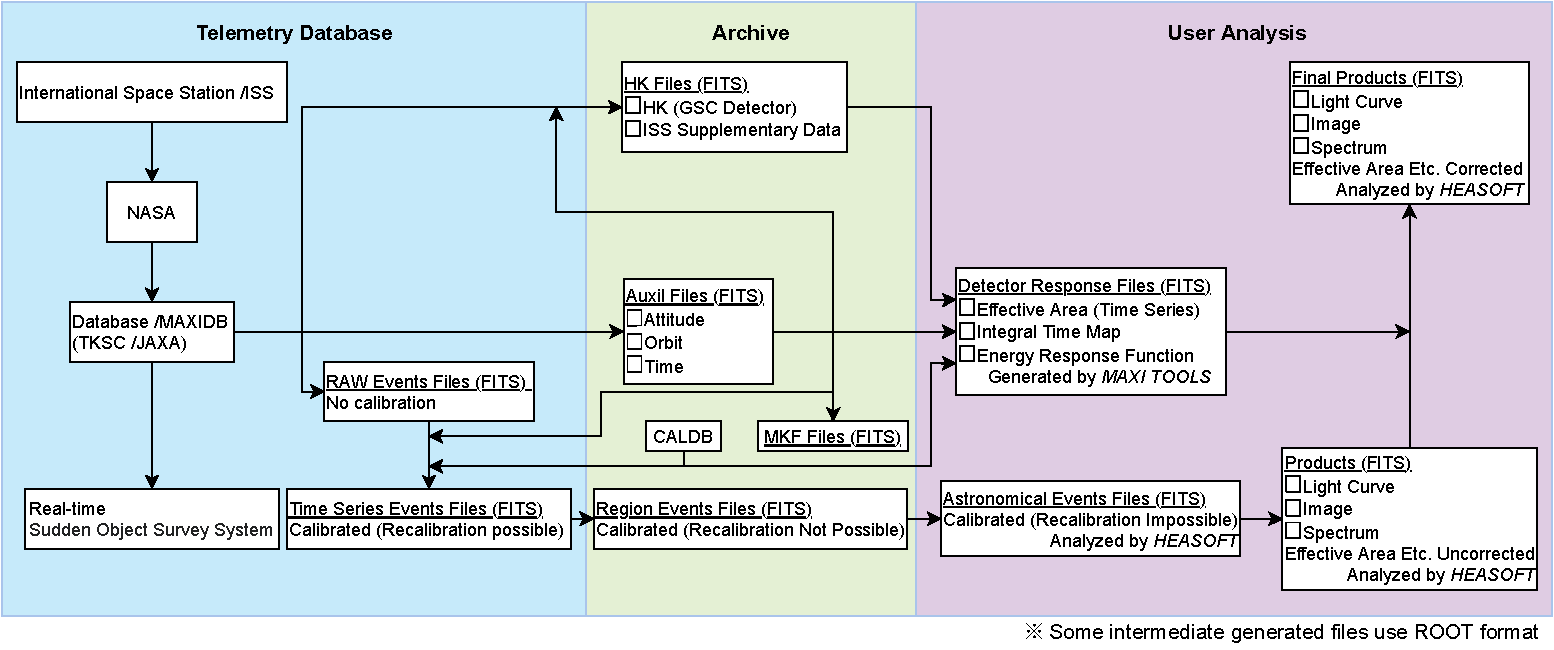
\includegraphics[width=1\textwidth]{1_1.pdf}
  \caption{The data flow and analysis flow of MAXI are shown above.}
  \label{fig:1.1}
\end{figure}

\clearpage

\chapter{Data File Types}\label{ch:2}

This chapter describes the data files used in MAXI standard analysis.\\

\section{GSC}\label{sec:2.1}

\subsection{DP Mode of Event File}\label{subsec:2.1.1}

There are two types of formats, 32-bit and 64-bit of DP Mode. The difference between them is the accuracy of time tagging: 1s for 32-bit, and 50 $\mu$s for 64-bit due to FRC (GSC-MDP 50$\mu$s Free-Run Clock Counter). Before September 30, 2009, low-speed systems were 32-bit and medium-speed systems were 64-bit, after that, both low-speed and medium-speed systems were basically 64-bit. However, the low-speed system may be 32-bit immediately after rebooting. In addition, Software LD/UD is different for low-speed and medium-speed systems. \\
\indent A 64-bit file can be converted to a 32-bit file. The Cleaned Event Files stored at RIKEN as described in \S\ref{sec:3.5} were converted from 64-bit to 32-bit for consistency with data prior to September 30, 2009. \\

\subsection{Raw Event File}\label{subsec:2.1.2}

This is a file with extracted Rev (Raw Event) data table from MAXI-DB and converted to fits binary table. It consists only of raw data from telemetry such as camera, anode, dptc, pha(L,R), etc. There is no distinction between A and B series in camera number. \\
\indent All the contents of Raw Event File are inherited by Processed Event File in subsequent stages, so the Raw Event File will not be returned in normal user analysis. \\

\subsection{Processed Event File}\label{subsec:2.1.3}

The raw event file is processed by adding time, coordinates, and PI using calibration data (CALDB) and auxiliary data (DPTC, Attitude, ...) of the detector, and then appended with columns like TIME, detx, bex, RA, DEC, X, Y, and PI. The cameraID is a serial number from 0-11. \\
\indent The file relies on the version of CALDB and Auxiliary Data. Reprocessing program mxgevt2evt can update the Processed Event File with the latest CALDB. \\
\indent RIKEN generates Processed Event File using the same slicing as Raw Event File, and then generates a file that is split by counter and summarized by day. \\

\subsection{Cleaned Event File}\label{subsec:2.1.4}

Processed Event File is filtered using HK. The conditions applied are as follows.
\begin{itemize}
  \item Edge cut ($|$DETX$|<$ 135.0mm)
  \item HV-on/off cut (15.0 sec $<$ T\_HV\_ON \&\& 15.0 sec $<$ TN\_HV\_OFF)
\end{itemize}
Since this is a loose condition, it is often better to apply a tight Filter in standard analysis. This is a starting point for Daily LC Analysis. \\

\subsection{HK File}\label{subsec:2.1.5}

A file that collects information about GSC power, HV monitor, LD count monitor, RBM monitor, count/RBM flags, etc., which is used for event selection in \texttt{xselect}. As long as there is no missing data, the steps are 1 second. \\
\indent Additionally, T\_HV\_ON (time from HV-on) and TN\_HV\_OFF (time until HV-off) are added. \\
\indent Generated daily by RIKEN's standard process. \\

\subsection{STDGTI}\label{subsec:2.1.6}

GTI Extension of the Cleaned Event File is extracted and compiled into a file. For normal astronomical analysis, STDGTI Extension HDU comes with the Event File is used. For special applications such as handling long-term all-sky data. \\
\indent Generated daily by RIKEN's standard process. \\

\section{SSC}\label{sec:2.2}


\subsection{Cleaned Event File}\label{subsec:2.2.1}

There are two types of formats: GRADE Format and PHA Format. \\

\section{Auxiliary File}\label{sec:2.3}

A file with auxiliary data such as ISS orbit, attitude, MAXI DP time clock, etc., which are required when analyzing observation data. It is placed in the directory \$MXSOFT/auxil. \\

\subsection{Time (DPTC)}\label{subsec:2.3.1}

DP time correction file (difference between DPTime and UTC), generated daily by JAXA. \\

\subsection{Attitude}\label{subsec:2.3.2}

MAXI attitude data, generated daily by JAXA. \\

\subsection{Orbit}\label{subsec:2.3.3}

ISS orbital data, generated daily by JAXA. \\

\subsection{MKF}\label{subsec:2.3.4}

A file with ISS latitude, longitude, altitude, cutoff-rigidity of Earth's magnetic field, and day/night information for each time of day, which is used for event selection (in xselect).\\
\indent Generated from Attitude, Orbit, and DPTC files.\\
\indent There is no arrangement to separate event selection parameter file from the HK file, but MKF assumes that it will be shared with SSC without depending on GSC counter information. \\
\indent It can be generated using MAXI software mxmkf, it is also generated daily by JAXA.\\

\subsection{ISSANC}\label{subsec:2.3.5}

Extracted data of solar paddle angle from ISS auxiliary file. There are two types: $\alpha$ and $\beta$ angle. It is used in program to determine the field-of-view shading. \\
\indent Generated daily by RIKEN's standard process. \\

\subsection{GSC-E FRC}\label{subsec:2.3.6}

A list of positive second values of DPTime from GSC MDP 20kHz (50$\mu$s) free-run clock counter, separated for group A and B. It is used in processing (time assigning) of 64-bit event data. \\
\indent Generated daily by RIKEN's standard process. \\

\section{CALDB File}\label{sec:2.4}

A file of calibration information of the instrument based on Heasarc CALDB (Calibration database) format. Managed and provided by the GSC and SSC teams separately. \\

\clearpage

\chapter{Preparation for Analysis}\label{ch:3}

This chapter explains how to compile and install the software libraries (\S\ref{sec:3.1}, \S\ref{sec:3.2}) necessary to start analysis, install and retrieve various data (\S\ref{sec:3.3}, \S\ref{sec:3.5}), and set environment variables (\S\ref{sec:3.6}) in turn. This section uses C shell environment as an example, so if you are using Bourne shell, please read this section differently as appropriate.\\

\section{Install External Software Libraries}\label{sec:3.1}

This section describes the procedure for compiling and installing external software libraries that are shown in Table \ref{tab:3.1}. If you want to retrieve event data directly from MAXI-DB, which means you want to use mxdbtool, please refer to \S \ref{appsec:1.1} and install Postgresql. Also, when using mxkwtool, please refer to \S \ref{appsec:1.1} and install fftw, gsl, and HEAsoft 6.12 before installing ROOT, and add options when configuring ROOT. In this section, we will assume that the downloaded source files are placed in "/opt/maxi/src", the work is done in "/opt/maxi/local\_20130505/install\_work" and will be installed in "/opt/maxi/local\_20130505". However, we will assume that only healpix is installed in the same directory ”/opt/maxi/mxsoft\_20130505” as MAXI software from \S\ref{sec:3.2}.\\

\begin{table}[hbtp!]
\caption{External software and libraries are shown below.}
\label{tab:3.1}
\centering
\begin{tabu} to \textwidth{lll}
\hline \hline
\textbf{Software} & \textbf{Version} & \textbf{Comment} \\
\hline
tcl-devel & -- & Install with yum or apt-get \\
tk-devel & -- & Install with yum or apt-get \\
readline-devel & -- & Install with yum or apt-get \\
pcre, pcre-devel & -- & Install with yum or apt-get, required for swig \\
openssl, openssl-devel & -- & Install with yum or apt-get, required for python (pyfits) \\
libtool  & -- & Required to use configure \\
\hline
python & 2.7.3 & -- \\
numpy & 1.6.2 & Required for pyfits \\
pyfits & 3.1 & python fits library \\
swig & 2.0.3 & Required for maxiutil \\
Postgresql  & 8.1 or 8.2 & Required for mxdbtool. See \S\ref{appsec:1.1} \\
fftw & 3.3.2 &  Required for mxkwtool. See \S\ref{appsec:1.1}\\
gsl & 1.15 & Required for mxkwtool. See \S\ref{appsec:1.1} \\
\hline
HEAsoft  & 6.13, 6.12 & 6.12 is required for mxkwtool. See \S\ref{appsec:1.1}. \\
ds9  & 7.1 & -- \\
ROOT    & v5.34.07 & Used in light curve correction script \\
Healpix  & 3.11 & Used in all-sky map \\
\hline
\end{tabu}
\end{table}

\

\noindent\underline{\textbf{tcl-devel, tk-devel, readline-devel, pcre, pcre-devel, openssl, openssl-devel, libtool}}\\

\noindent Here is an example to install using apt-get and yum. For some directory views like Ubuntu, you should use "dev" instead of "devel", so you need to be careful about the package name. \\

\noindent \$ apt-get install tcl-devel tk-devel readline-devel pcre pcre-devel openssl openssl-devel libtool\\
\$ yum install tcl-devel tk-devel readline-devel pcre pcre-devel openssl openssl-devel libtool\\

When compiling softwares in \S3.1 and \S3.2, depending on the environment in which configure is run, following error related to libtool may occur. \\

\begin{lstlisting}
checking build system type... Invalid configuration ‘/opt/maxi/local_20130505/
install_work/heasoft-6.12/x86_64-unknown-linux-gnu-libc2.12/lib’: machine
‘/opt/maxi/local_20130505/install_work/heasoft-6.12/x86_64-unknown-linux-gnu-libc2.12/lib’
not recognized configure: error: /bin/sh ./config.sub /opt/maxi/local_20130505/install_work/
heasoft-6.12/x86_64-unknown-linux-gnu-libc2.12/lib failed
\end{lstlisting}

\noindent If you get this error, it is possible that libtool is not installed. If it is installed, copy following files to the directory where configure exists, and run configure.\\

\noindent \$ cp /usr/share/libtool/config/config.guess .\\
\$ cp /usr/share/libtool/config/config.sub .\\

\

\noindent\underline{\textbf{python 2.7.3}} -- http://www.python.org/ftp/python/2.7.3/Python-2.7.3.tgz\\

\noindent After compiling (make), following message will be displayed. Make sure that "\_ssl" is not in the list after the message. If you see "\_ssl", it is possible that openssl and openssl-devel are not installed, so install them and compile python again. \\

\begin{lstlisting}[columns=fixed]
Python build finished, but the necessary bits to build these modules were not found:
bsddb185           dl                 gdbm
imageop            sunaudiodev
\end{lstlisting}

\noindent \$ cd /opt/maxi/local\_20130505/install\_work\\
\$ tar zxvf /opt/maxi/src/Python-2.7.3.tgz\\
\$ cd Python-2.7.3\\
\$ ./configure -{}-prefix=/opt/maxi/local\_20130505 -{}-enable-shared\\
\$ make\\
\$ make install\\
\$ pwd\\
\phantom{\$ }/opt/maxi/local\_20130505/install\_work/Python-2.7.3\\
\$ cd ../\\
\$ setenv PATH /opt/maxi/local\_20130505/bin:\$PATH \phantom{aa}[For CSH]\\
\$ setenv LD\_LIBRARY\_PATH /opt/maxi/local\_20130505/lib:\$LD\_LIBRARY\_PATH \phantom{aa}[For CSH]\\
\$ export PATH=/opt/maxi/local\_20130505/bin:\$PATH \phantom{aa}[For BASH]\\
\$ export LD\_LIBRARY\_PATH=/opt/maxi/local\_20130505/lib:\$LD\_LIBRARY\_PATH \phantom{aa}[For BASH]\\

\

\noindent\underline{\textbf{numpy 1.6.2}} -- http://sourceforge.net/projects/numpy/files/NumPy/1.6.2/numpy-1.6.2.tar.gz/download\\

\noindent \$ tar zxvf /opt/maxi/src/numpy-1.6.2.tar.gz\\
\$ cd numpy-1.6.2\\
\$ /opt/maxi/local\_20130505/bin/python setup.py build\\
\$ /opt/maxi/local\_20130505/bin/python setup.py install\\
\$ pwd\\
\phantom{\$ }/opt/maxi/local\_20130505/install\_work/numpy-1.6.2\\
\$ cd ../\\

\

\noindent\underline{\textbf{pyfits 3.1}} -- http://pypi.python.org/packages/source/p/pyfits/pyfits-3.1.2.tar.gz\\

\noindent If you get following error when compiling pyfits, it is possible that openssl and openssl-devel are not installed, so install them and compile again. \\

\noindent urllib2.URLError:!`urlopen error unknown url type: https?`\\

\noindent \$ tar zxvf /opt/maxi/src/pyfits-3.1.2.tar.gz\\
\$ cd pyfits-3.1.2\\
\$ /opt/maxi/local\_20130505/bin/python setup.py build\\
\$ /opt/maxi/local\_20130505/bin/python setup.py install\\
\$ pwd\\
\phantom{\$ }/opt/maxi/local\_20130505/install\_work/pyfits-3.1.2\\
\$ cd ../\\

\

\noindent\underline{\textbf{swig 2.0.3}} -- http://sourceforge.net/projects/swig/files/swig/swig-2.0.3/swig-2.0.3.tar.gz/download\\

\noindent \$ tar zxvf /opt/maxi/src/swig-2.0.3.tar.gz\\
\$ cd swig-2.0.3\\
\$ ./configure -{}-prefix=/opt/maxi/local\_20130505\\
\phantom{\$ }-{}-with-python=/opt/maxi/local\_20130505/bin/python -{}-without-python3\\
\$ make\\
\$ make install\\
\$ pwd\\
\phantom{\$ }/opt/maxi/local\_20130505/install\_work/swig-2.0.3\\
\$ cd ../\\

\

\noindent\underline{\textbf{HEAsoft 6.13}} -- http://heasarc.gsfc.nasa.gov/docs/software/lheasoft\footnote{If a new version is released, it can be obtained from "ftp://heasarc.gsfc.nasa.gov/software/lheasoft/lheasoft6.13". You can obtain heasoft-6.13 from this address via wget, or download heasoft-6.13src.tar.gz if it is available.}\\

\noindent Install HEAsoft from source. For packages, at least ASCA and Xspec should be selected. If you get an error about python while running make, check if the environment variables of python mentioned previously are set. \\

\noindent \$ tar zxvf heasoft-6.13src.tar.gz\\
\$ cd heasoft-6.13/BUILD\_DIR \$ ./configure $>$\& config.out\\
\$ make $>$\& build.log\\
\$ make install $>$\& install.log \\

\noindent For compiling of ROOT, you need to set environment variables as follows and create symbolic links. The following "x86\_64-unknown-linux-gnu-libc2.12" varys depending on the PC environment you are using, so please read it differently as appropriate (the same hereafter).\\

\noindent \$ setenv HEADAS /opt/maxi/local\_20130505/install\_work/heasoft-6.13/x86\_64-unknown-linux-gnu-libc2.12 \phantom{aa}[For CSH]\\
\$ source \$HEADAS/headas-init.csh \phantom{aa}[For CSH]\\
\$ export HEADAS=/opt/maxi/local\_20130505/install\_work/heasoft-6.13/x86\_64-unknown-linux-gnu-libc2.12
\phantom{aa}[For BASH]\\
\$ source \$HEADAS/headas-init.sh \phantom{aa}[For BASH]\\
\$ cd \$HEADAS/lib\\
\$ ln -s libcfitsio\_3.32.so libcfitsio.so\\
\$ pwd\\
\phantom{\$ }/opt/maxi/local\_20130505/install\_work/heasoft-6.13/x86\_64-unknown-linux-gnu-libc2.12/lib\\
\$ cd ../../../\\

\noindent To handle MAXI data in xselect, write following MAXI Mission parameter information in "\$HEADAS/bin/xselect.mdb".\\

\begin{lstlisting}[columns=fixed, basicstyle=\ttfamily\scriptsize]
!
! MAXI
!
MAXI:submkey       NONE
MAXI:instkey       INSTRUME
MAXI:dmodekey      DATAMODE
MAXI:mkf_def_expr  mx*.mkf*
MAXI:mkf_rel_dir   .
MAXI:time          TIME
MAXI:tunits        s
MAXI:binsize       16.
MAXI:x             X
MAXI:y             Y
MAXI:xsiz          TLMAX
MAXI:ysiz          TLMAX
MAXI:detx          DETX
MAXI:dety          DETY
MAXI:detxsiz       TLMAX
MAXI:detysiz       TLMAX
MAXI:rawx          NONE
MAXI:rawy          NONE
MAXI:rawxsiz       NONE
MAXI:rawysiz       NONE
MAXI:phamax        TLMAX
MAXI:gti           STDGTI
MAXI:events        EVENTS
MAXI:timeorder     yes
!MAXI:instruments  GSC SSC
MAXI:instruments   GSC GSC_0 GSC_1 GSC_2 GSC_3 GSC_4 GSC_5 GSC_6 GSC_7 GSC_8 GSC_9 GSC_A GSC_B SSC SSC_H SSC_Z
MAXI:spbn          1
MAXI:ecol          PI
MAXI:ccol          NONE
MAXI:gcol          NONE
MAXI:imagecoord    SKY
MAXI:wmapcoord     SKY
MAXI:catnum        1
MAXI:wtmapb        yes
MAXI:wtmapfix      no
MAXI:lststr        *.evt
MAXI:fbin          1
MAXI:hbin          1
MAXI:GSC:modes     64BIT 32BIT 16BIT
MAXI:SSC:modes     64BIT
MAXI:extract       extractor
MAXI:catcol        OBJECT TELESCOP INSTRUME DATAMODE DATE-OBS DATE-END TIME-OBS
MAXI:dispcol       OBJECT DATE-OBS DATE-END TIME-OBS
MAXI:extendresp    yes
\end{lstlisting}

\

\noindent\underline{\textbf{ds9 7.1}} -- http://hea-www.harvard.edu/RD/ds9/site/Download.html\footnote{Older versions can be obtained from "http://hea-www.harvard.edu/RD/ds9/archive".}\\

\noindent Determine whether you need the 64-bit or 32-bit version according to the PC environment you are using and install it. \\

\noindent \$ tar zxvf /opt/maxi/src/ds9.linux64.7.1.tar.gz -C /opt/maxi/local\_20130505/bin\\

\

\noindent\underline{\textbf{ROOT 5.34.07}} -- ftp://root.cern.ch/root/root\_v5.34.07.source.tar.gz\\

\noindent If you don't use mxkwtool, all configure options are not necessary. \\

\noindent \$ tar zxvf /opt/maxi/src/root\_v5.34.07.source.tar.gz\\
\$ mv root root\_v5.34.07\\
\$ cd root\_v5.34.07\\
\$ ./configure \\
\phantom{\$ }-{}-with-cfitsio-incdir=\$HEADAS/include\\
\phantom{\$ }-{}-with-cfitsio-libdir=\$HEADAS/lib\\
\phantom{\$ }-{}-with-python-incdir=/opt/maxi/local\_20130505/include/python2.7\\
\phantom{\$ }-{}-with-python-libdir=/opt/maxi/local\_20130505/lib\\
\$ make\\
\$ setenv ROOTSYS /opt/maxi/local\_20130505/install\_work/root\_v5.34.07 \phantom{aa}[For CSH]\\
\$ source \$ROOTSYS/bin/thisroot.csh \phantom{aa}[For CSH]\\
\$ export ROOTSYS=/opt/maxi/local\_20130505/install\_work/root\_v5.34.07 \phantom{aa}[For BASH]\\
\$ source \$ROOTSYS/bin/thisroot.sh \phantom{aa}[For BASH]\\
\$ pwd\\
\phantom{\$ }/opt/maxi/local\_20130505/install\_work/root\_v5.34.07\\
\$ cd ../\\

\

\noindent\underline{\textbf{healpix 3.11}} -- \\ http://sourceforge.net/projects/healpix/files/Healpix\_3.11/Healpix\_3.11\_2013Apr24.tar.gz/download\\

\noindent \$ setenv MXSOFT /opt/maxi/mxsoft\_20130505 \phantom{aa}[For CSH]\\
\$ export MXSOFT=/opt/maxi/mxsoft\_20130505 \phantom{aa}[For BASH]\\
\$ cd \$MXSOFT\\
\$ mkdir healpix\\
\$ cd healpix\\
\$ tar zxvf /opt/maxi/src/Healpix\_3.11\_2013Apr24.tar.gz\\
\$ cd Healpix\_3.11/src/C/subs\\
\$ sed 's/lcfitsio/lcfitsio 3.32/g' Makefile $>$ Makefile.local\\
\$ make -f Makefile.local shared OPT=-fPIC CFITSIO\_INCDIR=\$HEADAS/include CFITSIO\_LIBDIR=\$HEADAS/lib\\
\$ mkdir \$MXSOFT/include \$MXSOFT/lib\\
\$ make -f Makefile.local install LIBDIR=\$MXSOFT/lib INCDIR=\$MXSOFT/include\\
\$ pwd \\
\phantom{\$ }/opt/maxi/mxsoft\_20130505/healpix/Healpix\_3.11/src/C/subs\\
\$ cd ../../../../../\\

\section{Install MAXI Software}\label{sec:3.2}

This section describes the procedure for compiling and installing MAXI software using configure version\footnote{The version released by developer requires rewriting of Makefile.in, but Nakagawa (ISAS/JAXA) has prepared a version with an additional configure script for easy installation. The released version number is suffixed with "c".} shown in Table \ref{tab:3.2}. The development was done on Cent-OS 5.X x86\_64 (64-bit), and been tested on i386 (32-bit). Each MAXI software has its own version number, but they are also grouped together to give a version number, and Table \ref{tab:3.2} is for Ver.20130505. It still includes provisional versions by May 2013. If you want to get event data directly from MAXI-DB, install mxdbtool with reference to \S\ref{appsec:1.2}. If you want to perform positioning, install mxkwtool with reference to \S\ref{appsec:1.2}. Note that mxdbtool and mxkwtool should be installed after the other MAXI software is installed. Here, we assume that you want to install in "/opt/maxi/mxsoft\_20130505". As MAXI software must run with the version combination listed in Table \ref{tab:3.2}, which are checked by the configure script, the directory structure must be exactly the same as described in this section\footnote{The requirement to keep the directory structure exactly the same may be inconvenient, but it is also intended to deal with the fact that some header files are currently placed in, for example, "maxitool/3.26a/include" instead of "\$MXSOFT/include".}.\\
\indent The Subversion account is the same as Wiki account, and you need to specify username when you run "svn". In the following explanations, we will use "USERNAME" as username, so please replace it with your own username.\\
\indent Make sure that following environment variables are set. If they are not set, it will not affect configure, but it can vsimplify the procedure as explained below. If MXSOFT is defined, MXSOFT will be set in prefix when configure is executed. Also, if you set HEADAS and ROOT environment variables, you can omit various options in configure. \\

\noindent \$ setenv PATH /opt/maxi/local\_20130505/bin:\$PATH \phantom{aa}[For CSH]\\
\$ setenv LD\_LIBRARY\_PATH /opt/maxi/local\_20130505/lib:\$LD\_LIBRARY\_PATH \phantom{aa}[For CSH]\\
\$ setenv HEADAS /opt/maxi/local\_20130505/install\_work/heasoft-6.13/x86\_64-unknown-linux-gnu-libc2.12
\phantom{aa}[For CSH]\\
\$ source \$HEADAS/headas-init.csh \phantom{aa}[For CSH]\\
\$ setenv ROOTSYS /opt/maxi/local\_20130505/install\_work/root\_v5.34.07 \phantom{aa}[For CSH]\\
\$ source \$ROOTSYS/bin/thisroot.csh \$ROOTSYS \phantom{aa}[For CSH]\\
\$ setenv MXSOFT /opt/maxi/mxsoft\_20130505 \phantom{aa}[For CSH]\\

\noindent \$ export PATH=/opt/maxi/local\_20130505/bin:\$PATH \phantom{aa}[For BASH]\\
\$ export LD\_LIBRARY\_PATH=/opt/maxi/local\_20130505/lib:\$LD\_LIBRARY\_PATH \phantom{aa}[For BASH]\\
\$ export HEADAS=/opt/maxi/local\_20130505/install\_work/heasoft-6.13/x86\_64-unknown-linux-gnu-libc2.12
\phantom{aa}[For BASH]\\
\$ source \$HEADAS/headas-init.sh \phantom{aa}[For BASH]\\
\$ export ROOTSYS=/opt/maxi/local\_20130505/install\_work/root\_v5.34.07 \phantom{aa}[For BASH]\\
\$ source \$ROOTSYS/bin/thisroot.sh \phantom{aa}[For BASH]\\
\$ export MXSOFT=/opt/maxi/mxsoft\_20130505 \phantom{aa}[For BASH]\\

\begin{table}[hbtp!]
\caption{List of MAXI software (Ver.20130505).}
\label{tab:3.2}
\centering
\begin{tabu} to \textwidth{lll}
\hline \hline
\textbf{Software} & \textbf{Version} & \textbf{Comment} \\
\hline
maxitool  & 3.26a & -- \\
gsc software & 1.36.2a & -- \\
obsjud  & 0.2.2mx & - \\
maxiutil & 1.45a & -- \\
f2root & 0.5 & Tool to convert FITS format Event File to ROOT format \\
mxdbtool  & 2.0a & Tool to retrieve Event File from MAXI-DB in FITS format. See \S \ref{appsec:1.2}. \\
mxkwtool  & 2.1.2 & Positioning tools. See \S \ref{appsec:1.2}. \\
\hline
\end{tabu}
\end{table}

\

\noindent\underline{\textbf{maxitool 3.26a}} \\

\noindent \$ cd \$MXSOFT\\
\$ mkdir maxitool\\
\$ cd maxitool\\
\$ svn export -{}-username=USERNAME http://www.maxi.jaxa.jp/svnrepo\_mission/common/maxitool/branches/3.26a\_c\\
\$ cd 3.26a\_c\\
\$ ./configure\\
\$ make\\
\$ make install\\
\$ pwd\\
\phantom{\$ }/opt/maxi/mxsoft\_20130505/maxitool/3.26a\_c\\
\$ cd ../../\\

\

\noindent\underline{\textbf{gsc software 1.36.2a}} \\

\noindent \$ mkdir gsc\\
\$ cd gsc\\
\$ svn export -{}-username=USERNAME http://www.maxi.jaxa.jp/svnrepo\_mission/gsc/resp/branches/1.36.2a\_c\\
\$ cd 1.36.2a\_c\\
\$ ./configure\\
\$ make\\
\$ make install\\
\$ pwd\\
\phantom{\$ }/opt/maxi/mxsoft\_20130505/gsc/1.36.2a\_c\\
\$ cd ../../\\

\

\noindent\underline{\textbf{obsjud 0.2.2mx}} \\

\noindent \$ mkdir obsjud\\
\$ cd obsjud\\
\$ svn export -{}-username=USERNAME http://www.maxi.jaxa.jp/svnrepo\_mission/common/obsjud/branches/0.2.2mx\_c\\
\$ cd 0.2.2mx\_c\\
\$ ./configure\\
\$ make\\
\$ make install\\
\$ pwd\\
\phantom{\$ }/opt/maxi/mxsoft\_20130505/obsjud/0.2.2mx\_c\\
\$ cd ../../\\

\

\noindent\underline{\textbf{maxiutil 1.45a}} \\

\noindent \$ mkdir maxiutil\\
\$ cd maxiutil\\
\$ svn export -{}-username=USERNAME http://www.maxi.jaxa.jp/svnrepo\_mission/common/maxiutil/branches/1.45a\_c\\
\$ cd 1.45a\_c\\
\$ ./configure\\
\$ make\\
\$ make install\\
\$ pwd\\
\phantom{\$ }/opt/maxi/mxsoft\_20130505/maxiutil/1.45a\_c\\
\$ cd ../../\\

\

\noindent\underline{\textbf{f2root 0.5}} \\

\noindent \$ mkdir f2root\\
\$ cd f2root\\
\$ svn export -{}-username=USERNAME http://www.maxi.jaxa.jp/svnrepo\_mission/common/f2root/branches/0.5\_c\\
\$ cd 0.5\_c\\
\$ ./configure\\
\$ make\\
\$ make install\\
\$ pwd\\
\phantom{\$ }/opt/maxi/mxsoft\_20130505/f2root/0.5\_c\\
\$ cd ../../\\

\

\noindent\underline{\textbf{pfiles Symbolic Links}} \\

\noindent Create symbolic links for files in "\$MXSOFT/pfiles" to "\$HEADAS/syspfiles".\\

\noindent \$ cd \$HEADAS/syspfiles\\
\$ ln -s \$MXSOFT/pfiles/*.par .\\

\section{Install CALDB}\label{sec:3.3}

This section describes the procedure for installing CALDB as shown in Table \ref{tab:3.3}. Here, we assume that you want to install in "/opt/maxi/mycaldb\_20130225". \\

\begin{table}[hbtp!]
\caption{The CALDB list is shown below.}
\label{tab:3.3}
\centering
\begin{tabu} to \textwidth{llll}
\hline \hline
\textbf{Mission} & \textbf{Detector} & \textbf{Version}& \textbf{Comment} \\
\hline
(Setup)  & -- & --& CALDB Setup Files \\
(Generic) & -- & --&  \\
MAXI & MIS & 20090809 & \\
MAXI & GSC & 20130225& \\
MAXI & SSC & 20111205 & \\
\hline
\end{tabu}
\end{table}

\

\noindent\underline{\textbf{Setup Files}} -- http://heasarc.gsfc.nasa.gov/FTP/caldb/software/tools/caldb\_setup\_files.tar.Z \\

\noindent \$ cd /opt/maxi/mycaldb\_20130225 \\
\$ tar zxvf /opt/maxi/src/caldb\_setup\_files.tar.Z\\

\noindent Rewrite this part of caldbinit.csh (or caldbinit.sh for Bourne shells) under "/opt/maxi/mycaldb\_20130225/software/tools" which configures CALDB. \\

\noindent Before : setenv CALDB /FTP/caldb \phantom{aa}[For CSH]\\
After\phantom{/} : setenv CALDB /opt/maxi/mycaldb\_20130225 \phantom{aa}[For CSH]\\

\noindent Before : export CALDB=/FTP/caldb \phantom{aa}[For BASH]\\
After\phantom{/} : export CALDB=/opt/maxi/mycaldb\_20130225 \phantom{aa}[For BASH]\\

\noindent Add the following part to "/opt/maxi/mycaldb\_20130225/software/tools/caldb.config". \\

\begin{lstlisting}
#
# MAXI
#
MAXI GSC    CALDB  data/maxi/gsc  caldb.indx  CALDB  data/maxi/gsc
MAXI GSC_0  CALDB  data/maxi/gsc  caldb.indx  CALDB  data/maxi/gsc
MAXI GSC_1  CALDB  data/maxi/gsc  caldb.indx  CALDB  data/maxi/gsc
MAXI GSC_2  CALDB  data/maxi/gsc  caldb.indx  CALDB  data/maxi/gsc
MAXI GSC_3  CALDB  data/maxi/gsc  caldb.indx  CALDB  data/maxi/gsc
MAXI GSC_4  CALDB  data/maxi/gsc  caldb.indx  CALDB  data/maxi/gsc
MAXI GSC_5  CALDB  data/maxi/gsc  caldb.indx  CALDB  data/maxi/gsc
MAXI GSC_6  CALDB  data/maxi/gsc  caldb.indx  CALDB  data/maxi/gsc
MAXI GSC_7  CALDB  data/maxi/gsc  caldb.indx  CALDB  data/maxi/gsc
MAXI GSC_8  CALDB  data/maxi/gsc  caldb.indx  CALDB  data/maxi/gsc
MAXI GSC_9  CALDB  data/maxi/gsc  caldb.indx  CALDB  data/maxi/gsc
MAXI GSC_A  CALDB  data/maxi/gsc  caldb.indx  CALDB  data/maxi/gsc
MAXI GSC_B  CALDB  data/maxi/gsc  caldb.indx  CALDB  data/maxi/gsc
#
MAXI SSC    CALDB  data/maxi/ssc  caldb.indx  CALDB  data/maxi/ssc
MAXI SSC_H  CALDB  data/maxi/ssc  caldb.indx  CALDB  data/maxi/ssc
MAXI SSC_Z  CALDB  data/maxi/ssc  caldb.indx  CALDB  data/maxi/ssc
#
MAXI VSC    CALDB  data/maxi/mis  caldb.indx  CALDB  data/maxi/mis
MAXI INS    CALDB  data/maxi/mis  caldb.indx  CALDB  data/maxi/mis
\end{lstlisting}

\

\noindent\underline{\textbf{Generic}} -- http://heasarc.gsfc.nasa.gov/FTP/caldb/data/gen/goodfiles\_gen\_ins\_20120127.tar.Z \\

\noindent \$ tar zxvf /opt/maxi/src/goodfiles\_gen\_ins\_20120127.tar.Z \\

\

\noindent\underline{\textbf{MAXI/MIS}} -- \\
\tiny http://www.maxi.jaxa.jp/pm/mission\_team/pukiwiki/index.php?plugin=attach\&refer=MaxiSoft\%2Fmaxi\_caldb\&openfile=caldb\_maxi\_mis\_ht20090809.tar.gz \\

\noindent\normalsize \$ tar zxvf /opt/maxi/src/caldb\_maxi\_mis\_ht20090809.tar.gz \\

\

\noindent\underline{\textbf{MAXI/GSC}} -- \\
http://www.maxi.jaxa.jp/pm/mission\_team/web/sugizaki/maxi/caldb\_archive/caldb\_maxi\_gsc\_ms20130225.tar.gz\\

\noindent \$ tar zxvf /opt/maxi/src/caldb\_maxi\_gsc\_ms20130225.tar.gz\\

\

\noindent\underline{\textbf{MAXI/SSC}} -- \\
\scriptsize http://www.maxi.jaxa.jp/pm/mission\_team/pukiwiki/index.php?plugin=attach\&refer=MaxiSoft\%2Fmaxi\_caldb\&openfile=ssc\_caldb\_20111205.tgz\\

\noindent\normalsize \$ cd data/maxi\\
\$ tar zxvf /opt/maxi/src/ssc\_caldb\_20111205.tgz\\

\

\noindent\underline{\textbf{Set Environment Variables}}\\

\noindent Execute the following command to set the environment variables for CALDB.\\

\noindent \$ source /opt/maxi/mycaldb\_20130225/software/tools/caldbinit.csh  \phantom{aa}[For CSH]\\

\noindent \$ source /opt/maxi/mycaldb\_20130225/software/tools/caldbinit.sh  \phantom{aa}[For BASH]\\

\

\section{Retrieve GSC RMF Database}\label{sec:3.4}

The GSC RMF Database is ready for each HV, each core line, and each detx, with disk capacity of about 110 GB. It is needed to run RMF Builder, which is used for spectral analysis of GSC. If you don't want to analyze GSC spectra, you don't need to get it. The data will be retrieved from following location at RIKEN. Contact the person in charge at RIKEN for access method. In this example, it is placed in "/opt/maxi/gscrmfdb". \\

\noindent gsc\at maxireceive.riken.jp:/dx1/gscrmfdb \\

Rewrite gscrmfdbidx.fits in the index file directly under gscrmfdb to match your PC environment. Specifically, you need to rewrite FILEDIR, which can be done in fparkey\_filedir.sh located directly under "gscrmfdb". Change the content of fparkey\_filedir.sh as below. \\

\noindent Before : /opt/gscrmfdb \\
After\phantom{/} : /opt/maxi/gscrmfdb \\

\noindent Execute following commands. \\

\noindent \$ cd /opt/maxi/gscrmfdb\\
\$ ./fparkey\_filedir.sh\\

\noindent Set environment variables like below. \\

\noindent \$ setenv GSCRMFDB /opt/maxi/gscrmfdb  \phantom{aa}[For CSH]\\

\noindent \$ export GSCRMFDB=/opt/maxi/gscrmfdb  \phantom{aa}[For BASH]\\

\section{Retrieve Cleaned Event File and Auxiliary File}\label{sec:3.5}

You can retrieve GSC Cleaned Event File and Auxiliary File from following locations at RIKEN. Contact the relevant person at RIKEN for access method (password). Since they are daily updated, it is convenient to rsync with cron. In this example, they are placed in "/opt/maxi/mxdata". \\

\noindent gsc\at maxireceive.riken.jp:/dx1/mxdata\_jax/gsc.v1.4 \\
gsc\at maxireceive.riken.jp:/dx1/mxdata\_jax/auxil \\
gsc\at maxireceive.riken.jp:/dx1/mxdata\_jax/mkf \\
gsc\at maxireceive.riken.jp:/dx1/mxdata\_jax/rbmhk \\

\noindent Rewrite FILEDIR of index file directly under auxil to "/opt/maxi/mxdata". It can be rewritten using fparkey contained in HEAsoft, by excuting following commands.\\

\noindent \$ fparkey /opt/maxi/mxdata attlist.fits FILEDIR\\
\$ fparkey /opt/maxi/mxdata dptclist.fits FILEDIR\\
\$ fparkey /opt/maxi/mxdata geafrclist.fits FILEDIR\\
\$ fparkey /opt/maxi/mxdata gebfrclist.fits FILEDIR\\
\$ fparkey /opt/maxi/mxdata issancpm.fits FILEDIR\\
\$ fparkey /opt/maxi/mxdata issancpmlist.fits FILEDIR\\
\$ fparkey /opt/maxi/mxdata issancsarj.fits FILEDIR\\
\$ fparkey /opt/maxi/mxdata issancsarjlist.fits FILEDIR\\
\$ fparkey /opt/maxi/mxdata orblist.fits FILEDIR\\

\noindent Finally, set environment variables as below.\\

\noindent \$ setenv MXDATA /opt/maxi/mxdata  \phantom{aa}[For CSH]\\

\noindent \$ export MXDATA=/opt/maxi/mxdata  \phantom{aa}[For BASH]\\

\section{Setup Script}\label{sec:3.6}

In \S\ref{sec:3.1}$\sim$\S\ref{sec:3.5}, we set the environment variables necessary to run MAXI software while compiling and installing. The setup script that summarizes them is shown below. If you want to use mxkwtool, remove the comment-out (\#) from the last 8 lines. Also, since mxkwtool uses not only HEAsoft 6.13, but also HEAsoft 6.12 for the libraries related to WCS, if you do not set up the environment variables as described in this setup script, you may get errors related to libraries in all MAXI software\footnote{Basically, MAXI software is compiled with HEAsoft 6.13, so when setting LD\_LIBRARY\_PATH, if you write HEAsoft 6.12 first, you will get an error due to difference in library versions.}.\\

\noindent\underline{\textbf{CSH Setup Script}}\\

\begin{lstlisting}[basicstyle=\ttfamily\small]
#================================================================
# Setup File for MAXI Software Ver.20130505
#================================================================
#
# set versions
setenv MXSOFT_VER 20130505
setenv HEADAS_VER 6.13
setenv CALDB_VER 20130225
setenv ROOT_VER v5.34.07
#
# set path
setenv PATH /usr/local/bin:/usr/bin:/bin
setenv LD_LIBRARY_PATH /usr/local/lib
#
# heasoft
setenv HEADAS /opt/maxi/local_20130505/install_work/heasoft-$HEADAS_VER/x86_64-unknown-linux-gnu-libc2.12
source $HEADAS/headas-init.csh
#
# root
source /opt/maxi/local_20130505/install_work/root_${ROOT_VER}/bin/thisroot.csh
#
# caldb
source /opt/maxi/mycaldb_$CALDB_VER/software/tools/caldbinit.csh
#
# mxsoft
setenv MXSOFT /opt/maxi/mxsoft_$MXSOFT_VER
setenv PATH $MXSOFT/bin:$PATH
setenv LD_LIBRARY_PATH $MXSOFT/lib:$LD_LIBRARY_PATH
setenv PFILES "$HOME/pfiles;$MXSOFT/pfiles:$HEADAS/syspfiles"
#
# mxdata
setenv MXDATA /opt/maxi/mxdata
setenv GSCRMFDB /opt/maxi/gscrmfdb
#
# python
setenv PYTHONPATH $MXSOFT/pylib:$PYTHONPATH
#
# mxkwtool
#setenv PATH $MXSOFT/mxkwtool/2.1.2/script:$PATH
#setenv MXKWTOOL $MXSOFT/mxkwtool/2.1.2
#setenv MXKW_TMPDIR $HOME/maxi/tmp
#setenv MXKW_DS9_BIN_DIR /opt/maxi/local_20130505/bin
#setenv MXKW_MXFILE_BUSY_FLAG $HOME/maxi/exec_flag_rsync_jax_data_from_riken
#setenv MXKW_GRBTOOL_CAT $MXSOFT/catalog/weblistv6_detect091209_merge_t.csv
#setenv MXKW_GRBTOOL_CAT_LOCAL $HOME/maxi/srcinfo.list
#setenv LD_LIBRARY_PATH {$LD_LIBRARY_PATH}:/opt/heasoft/6.12/x86_64-unknown-linux-gnu-libc2.12/lib
\end{lstlisting}

\

\noindent\underline{\textbf{BASH Setup Script}}\\

\begin{lstlisting}[basicstyle=\ttfamily\small]
#================================================================
# Setup File for MAXI Software Ver.20130505
#================================================================
#
# set versions
export MXSOFT_VER=20130505
export HEADAS_VER=6.13
export CALDB_VER=20130225
export ROOT_VER=v5.34.07
#
# set path
export PATH=/usr/local/bin:/usr/bin:/bin
export LD_LIBRARY_PATH=/usr/local/lib
#
# heasoft
export HEADAS=/opt/maxi/local_20130505/install_work/heasoft-$HEADAS_VER/x86_64-unknown-linux-gnu-libc2.12
source $HEADAS/headas-init.sh
#
# root
source /opt/maxi/local_20130505/install_work/root_${ROOT_VER}/bin/thisroot.sh
#
# caldb
source /opt/maxi/mycaldb_$CALDB_VER/software/tools/caldbinit.sh
#
# mxsoft
export MXSOFT=/opt/maxi/mxsoft_$MXSOFT_VER
export PATH=$MXSOFT/bin:$PATH
export LD_LIBRARY_PATH=$MXSOFT/lib:$LD_LIBRARY_PATH
export PFILES="$HOME/pfiles;$MXSOFT/pfiles:$HEADAS/syspfiles"
#
# mxdata
export MXDATA=/opt/maxi/mxdata
export GSCRMFDB=/opt/maxi/gscrmfdb
#
# python
export PYTHONPATH=$MXSOFT/pylib:$PYTHONPATH
#
# mxkwtool
#export PATH=$MXSOFT/mxkwtool/2.1.2/script:$PATH
#export MXKWTOOL=$MXSOFT/mxkwtool/2.1.2
#export MXKW_TMPDIR=$HOME/maxi/tmp
#export MXKW_DS9_BIN_DIR=/opt/maxi/local_20130505/bin
#export MXKW_MXFILE_BUSY_FLAG=$HOME/maxi/exec_flag_rsync_jax_data_from_riken
#export MXKW_GRBTOOL_CAT=$MXSOFT/catalog/weblistv6_detect091209_merge_t.csv
#export MXKW_GRBTOOL_CAT_LOCAL=$HOME/maxi/srcinfo.list
#export LD_LIBRARY_PATH={$LD_LIBRARY_PATH}:/opt/heasoft/6.12/x86_64-unknown-linux-gnu-libc2.12/lib
\end{lstlisting}

\clearpage

\chapter{Standard Analysis}\label{ch:4}

In this chapter we will explain the procedure to perform standard analysis of objects using the Cleaned Event File (\S\ref{sec:3.5}) generated by RIKEN. Since the procedures are almost the same for GSC and SSC, they are explained in parallel. In the case of Quick Look analysis, Event File is extracted directly from MAXI-DB, and after retrieving the Event File, the procedure is the same as in this chapter. \\

\section{Extract Event Files Around the Object}\label{sec:4.1}

You can generate Event File around the object by specifying centeral coordinate, surrounding radius, and XY Pixel Format from the all-sky data accumulated from time series for each camera. The program is \texttt{mxextract} for GSC and \texttt{mxsextract} for SSC. The way to use them is almost the same, but SSC's \texttt{mxsextract} has a parameter \texttt{outform} at the end to specify the format of output file. \\
\indent The XY coordinates of the output file will be reassigned in TAN Projection according to specified Pixel Format. If there has no Event that match the conditions, no Event File will be generated. The STDGTI Extension is inherited from Event File in the input files.\\
\indent When running, enter following parameters. \\

\noindent \texttt{infname}: The input file name (e.g. gsc0\_evtfile.fits) or file name list (e.g. evtfile.list). If you want to load multiple Event Files, you can list those file names in a text file, and enter \at evtfile.list in the input file section, then it will load files in the order listed. It is possible to process a list of Event Files from different cameras at once, but for now, STDGTI Extension does not process them correctly, so process each camera individually. \\

\noindent \texttt{outfname}: Name of the output file (fits binary table). \\

\noindent \texttt{ra}: Target Right Ascension (degree). \\

\noindent \texttt{dec}: Target Declination (degree). \\

\noindent \texttt{radi\_i}: Extraction inner radius. Normally, 0$^{\circ}$ is specified.\\

\noindent \texttt{radi\_o}: Extraction inner and outer diameter. It is recommended to use 8$^{\circ}$ larger than PSF to get the background region for light curve and spectrum analysis. \\

\noindent \texttt{nx}: X Pixel number of XY projection coordinates.\\

\noindent \texttt{ny}: Y Pixel number of XY projection coordinates.\\

\noindent \texttt{pixsize}:Pixel size of the XY projection coordinates (degree/pixel).\\

\noindent \texttt{attlist}: File name of posture file list. If it is installed in a predetermined location with a predetermined name, just put DEF. \\

\noindent \texttt{outform}: \underline{SSC only} Output event file format. 10: GRADE, 11: PHA, 20: EXT. EXT is PHA format with an additional parameter represents the angle of separation from the moon for each event. \\

For example, an execution script is as below. \\

\noindent\textbf{For GSC}\\
\begin{lstlisting}
#!/bin/sh
mjd=55501
gscid=4
infname="/nfs/m/maxir1/jax_data/rev1.1/low/evt_camid_cl/low32/gsc${gscid}_r2pcl_MJD${mjd}.evt"
outfname="crab_gsc${gscid}_mjd${mjd}.evt"
object="Crab"
ra=83.63
dec=22.01
radi_i=0.0
radi_o=10.0
nx=200
ny=200
pixsize=0.1
attlist="DEF"

mxextract $infname $outfname $object $ra $dec $radi_i $radi_o $nx $ny $pixsize $attlist
\end{lstlisting}

\

\noindent\textbf{For SSC}\\
\begin{lstlisting}
#!/bin/sh
mjd=55501
hz="h"
infname="/nfs/m/maxir1/ssc/evt_cleaned/ssc${hz}_allcl_mjd${mjd}.evt"
outfname="crab_ssc${hz}_mjd${mjd}.evt"
object="Crab"
ra=83.63
dec=22.01
radi_i=0.0
radi_o=10.0
nx=200
ny=200
pixsize=0.1
attlist="DEF"
outform=20

mxsextract $infname $outfname $object $ra $dec $radi_i $radi_o $nx $ny $pixsize $attlist $outform
\end{lstlisting}

\

The generated Event File is in FITS format, but it need to be converted from FITS format to ROOT format using \texttt{ftbl2root} to be analyzed by tools running ROOT Library. \\

\begin{lstlisting}
$ ftbl2root (fits file name) (root file name)
\end{lstlisting}

\

\section{Generate and Display Image File}\label{sec:4.2}

You can execute following commands (some parts are omitted for the sake of clarity) to load the Event File generated in \S\ref{sec:4.1} with \texttt{xselect}, generate Image, display with ds9, and save it. If you load more than one Event File at a time, you will get an accumulated image. If you want to load multiple Event Files, create a Event File list in text format (e.g., evtfile.list) and specify "\at evtfile.list" instead of name of Event Files. Also, if you want to specify the energy band, set "pha\_cutoff"\footnote{The relationship between energy ($E$) and channel ($N$) is $E = 50N$ [eV].}. \\

\begin{lstlisting}
$ xselect

> Enter session name >[]gsc4
gsc4:SUZAKU > read events crab_gsc4_mjd55501.evt <-- (* Or "\at evtfile.list". *)
> Enter the Event file dir >[.] .
Got new mission: MAXI
> Reset the mission ? >[yes] yes

gsc4:MAXI-GSC-32BIT > filter pha_cutoff 40 200 <-- (* Set energy band to 2-10 keV. *)
gsc4:MAXI-GSC-32BIT > extract image <-- (* Generate Image. *)
gsc4:MAXI-GSC-32BIT > sao <-- (* Display in ds9. *)
gsc4:MAXI-GSC-32BIT > save image crab_gsc4_mjd55501_2_10keV.img <-- (* Save the file. *)
\end{lstlisting}

\

\begin{figure}[hbtp!]
  \centering
  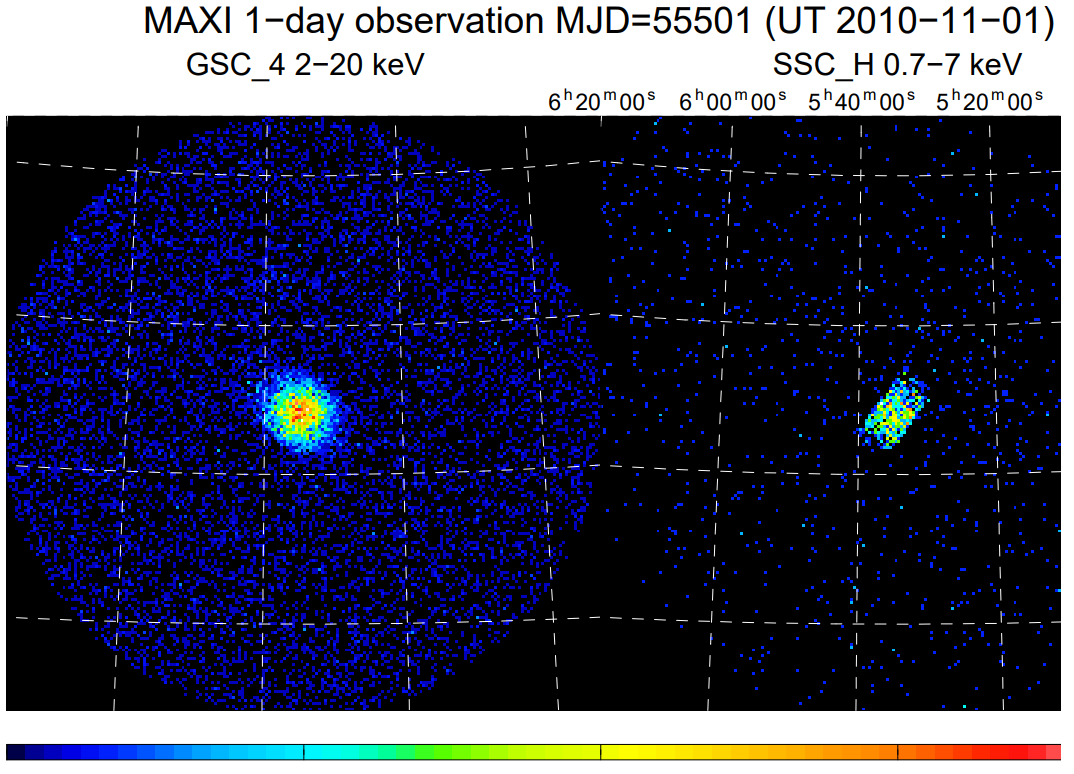
\includegraphics[width=0.8\textwidth]{4_1.png}
  \caption{The image of integrated Crab for one day on November 1, 2010 is shown. The left figure shows the 2-20 keV image of GSC-4, the right figure shows the 0.7-7 keV image of SSC-H.}
  \label{fig:1}
\end{figure}

\section{Light Curve Analysis}\label{sec:4.3}

This section describes the procedure to correct observation time, effective area, and background, in order to derive a light curve with time scale larger than MAXI orbit scan period ($\sim$90 min) for an X-ray source with known coordinates. \\

\subsection{Determine How to Estimate the Background Level}\label{subsec:4.3.1}

Look at the image generated in \S\ref{sec:4.2} and decide how to estimate the background level. There are two ways to do so. \\

\noindent \textbf{Without contamination source near the target} \\

You can estimate the background rate in the source from event rate before and after the source enters the field of view of detecting region, with the same collimator incidence angle for each scan. From which area to estimate the source event rate and background rate is clarified in the process in \S \ref{subsec:4.3.3}. Figure \ref{fig:4.2} shows the parameters to define region. \\

\begin{figure}[hbtp!]
  \centering
  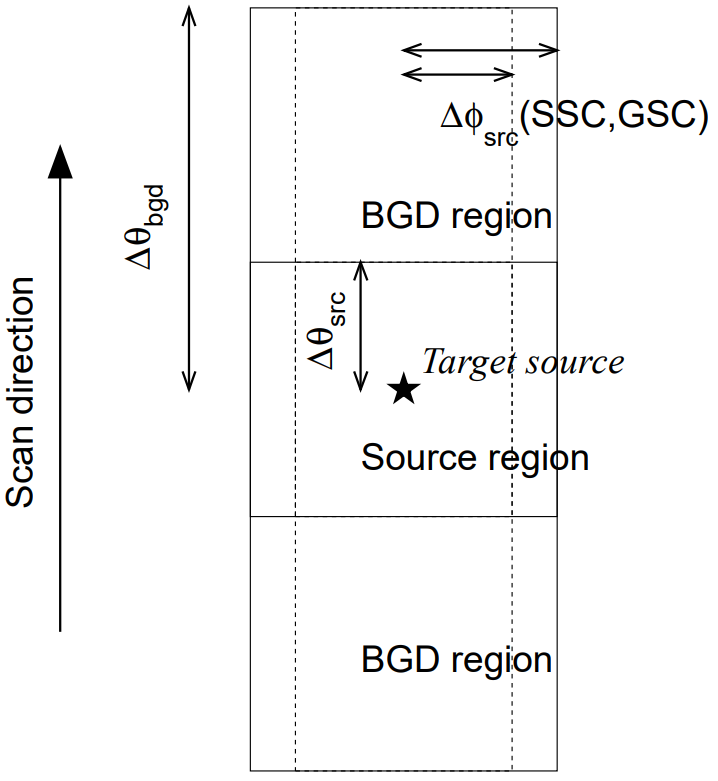
\includegraphics[width=0.4\textwidth]{4_2.png}
  \caption{Parameters to be used when estimating the background from the event rate before and after the target enters the field of view of detecting region. Define the source and background regions using the collimator incidence angle spherical coordinates ($\theta_{\text{col}},\phi_{\text{col}}$) and the separation angle from the target. $\Delta\phi_{\text{src}}$ (\texttt{srcreg\underline{ }dcolphi}), $\Delta\theta_{\text{src}}$ (\texttt{srcreg\underline{ }dcoltha}), $\Delta\theta_{\text{bgd}}$ (\texttt{bgdreg\underline{ }dcoltha})}
  \label{fig:4.2}
\end{figure}

\noindent \textbf{With contamination source near the target} \\

You can use celestial coordinates to determine the source and background regions, and assume that the background is uniform per solid angle, then estimate background rate in the source. To do so, first create Region File for source region and background region respectively (here the file names are src.reg and bkg.reg). Plot the image generated in \S\ref{sec:4.2} in ds9, determine Region\footnote{I won't go into details about the Region, as there is plenty of information about it on the Internet, but for example, the Suzaku satellite's "First Step Guide" (http://cosmic.riken.jp/suzaku/help/guide/fstep\_web/node8.html) is a good reference.}, and save it in SKYXY coordinates (Format: ds9, Coordinates: fk5). \\
\indent Read the Event File around the body generated in \S\ref{sec:4.1} with xselect, and then read the created Region File to generate Event File for source and background regions respectively. An example of working with xselect is shown below. The Event File should be converted from FITS format to ROOT format using ftbl2root as described in \S\ref{sec:4.1}. Unless it is a special Region File, the areas of source and background regions are described in the "Header Key Parameter: NPIXSOU" of the extracted Event File.\\

\begin{lstlisting}
$ xselect

> Enter session name >[]gsc4
gsc4:SUZAKU > read events crab_gsc4_mjd55501.evt
> Enter the Event file dir >[.] .
Got new mission: MAXI
> Reset the mission ? >[yes] yes

gsc4:MAXI-GSC-32BIT > set XYNAME X Y

gsc4:MAXI-GSC-32BIT > filter region src.reg
gsc4:MAXI-GSC-32BIT > extract events
gsc4:MAXI-GSC-32BIT > save events crab_gsc4_mjd55501_src.evt
> Use filtered events as input data file ? >[yes] no
gsc4:MAXI-GSC-32BIT > clear events
gsc4:MAXI-GSC-32BIT > clear region

gsc4:MAXI-GSC-32BIT > filter region bkg.reg
gsc4:MAXI-GSC-32BIT > extract events
gsc4:MAXI-GSC-32BIT > save events crab_gsc4_mjd55501_bkg.evt
> Use filtered events as input data file ? >[yes] no
gsc4:MAXI-GSC-32BIT > clear events
gsc4:MAXI-GSC-32BIT > clear region
\end{lstlisting}

\

\subsection{Generate Observation Condition File}\label{subsec:4.3.2}

You need to create an observation condition file (OBSCUR file) for the object to be analyzed. The program is the same for GSC and SSC, using \texttt{mxobscur}. \texttt{mxobscur} reads CALDB data, GTI data, attitude data, ISS paddle rotation angle, and field of view analysis library parameter\footnote{If you put NONE in the parameter of view analysis library, you can skip the paddle shielding determination.}, calculates the data shown in Table \ref{tab:4.1} for each camera, and then saves in FITS file. A maximum of 12 Extension HDUs are stored in a single FITS file for GSC (\texttt{instr=gsc}) and a maximum of 2 Extension HDUs are stored in a single FITS file for SSC (\texttt{instr=ssc})\footnote{This is different from the previous \texttt{mxgeaobscur} and \texttt{mxseaobscur}.}. If you specify a value such as "gtifile0=NONE", the camera will not be calculated and the Extension HDU will be reduced by that value.\\

\begin{table}[hbtp!]
\caption{The parameter name included in the table data of the observation condition file (OBSCUR file) is shown below.}
\label{tab:4.1}
\centering
\begin{tabu} to \textwidth{l|l}
\hline
TIME & MAXI Time\\
\makecell{GTI\\ \phantom{aaaaa}} & \makecell[l]{1 if TIME is in good time interval of the GTI file,\\ 0 otherwise, or 255 if it is out of the GTI file range.} \\
\makecell{OBSJUD\\ \phantom{aaaaa}} & \makecell[l]{The value returned by the visual field determination library.\\ 0 if the target is not hidden by shader.} \\
COLTHA & Collimtor Theta angle of the object. \\
COLPHI & Collimtor Phi angle of the object. \\
AREA & Collimator Area relative to the angle of incidence of the object. \\
\hline
\end{tabu}
\end{table}

\

The input parameters are as follows. \\

\noindent \texttt{instr}: GSC or SSC. \\

\noindent \texttt{outfname}: Output observation condition file name. FITS file. \\

\noindent \texttt{ra}: Right Ascension (degree) of the target. \\

\noindent \texttt{dec}: Declination (degree) of the target. \\

\noindent \texttt{tstart}: Observation start time (MJD).\\

\noindent \texttt{tstop}: Observation end time (MJD). \\

\noindent \texttt{dt}: Calculation time step (seconds). Normally 1 (seconds).\\

\noindent \texttt{colphi\underline{ }max}: Upper limit of the source incidence angle $|\phi_{\text{col}}|$ of results to output to thr file. The source is considered to be out of the field of view if it is larger than this value and will not be saved. About 42$^{\circ}$ for GSC and 46$^\circ$ for SSC.\\

\noindent \texttt{coltha\underline{ }max}: Upper limit of the source incidence angle $|\theta_{\text{col}}|$ of results to output to thr file. Since it will be used later to calculate the exposure respect to the background and the source, it should be slightly larger than the field of view with up to about 8$^\circ$.\\

\noindent \texttt{attlist}:  The file name of the posture file list. Normally, DEF is specified. \\

\noindent \texttt{obsjud\underline{ }dname}: Name of the directory where the parameter files for visual field analysis library are located. The order of parameters has changed since ver.1.0. Normally, DEF is enough to use. If NONE is entered, the field-of-view determination calculation is skipped. \\

\noindent \texttt{sarjfnamelist}: List file name for solar paddle $\alpha$ angle. Normally, DEF is specified. \\

\noindent \texttt{pmfnamelist}: List file name for solar paddle  $\beta$ angle. Normally, DEF is specified.\\

\noindent \texttt{gtifile0, .\!.\!., gtifile11}: Set GTI file name for each camera. The GTI File is in FITS format, and is assumed to have the same format as the STDGTI Extension HDU in Event File. Normally, this will be specified as Event File. For GSC (\texttt{instr=gsc}), 12 input parameters \texttt{gtifile0, ..., gtifile11} will be read. For SSC (\texttt{instr=ssc}), only the first two (gtifile0: SSC-H, gtifile1: SSC-Z) will be read. If there is no GTI File, or if data of a camera is not to be used for further analysis, set "NONE". For GSC, there are daily generated files that extracts only the STDGTI of all Cleaned Event Files for each camera. \\

\noindent \textbf{Execution script sample for GSC} \\

\begin{lstlisting}[frame=single]

#!/bin/sh

mjd=55058
mjd_end=55059

instr=gsc  (* \# For SSC, this field should be set to "ssc". *)
outfname=crab_gobscur_mjd${mjd}.fits

ra=83.63
dec=22.01
tstart=$mjd
tstop=$mjd_end
dt=1.0
colphi_max=42.0
coltha_max=10.0
attlist=DEF
obsjud_dname=DEF
sarjfnamelist=DEF
pmfnamelist=DEF

gtifile0=NONE
gtifile1=crab_gsc1_mjd${mjd}.evt
gtifile2=crab_gsc2_mjd${mjd}.evt
gtifile3=NONE
gtifile4=crab_gsc4_mjd${mjd}.evt
gtifile5=crab_gsc5_mjd${mjd}.evt
gtifile6=NONE
gtifile7=crab_gsc7_mjd${mjd}.evt
gtifile8=crab_gsc8_mjd${mjd}.evt
gtifile9=NONE
gtifilea=crab_gsca_mjd${mjd}.evt
gtifileb=crab_gscb_mjd${mjd}.evt

cmdstr="mxobscur $instr $outfname $ra $dec $tstart $tstop $dt $colphi_max $coltha_max \
 $attlist $obsjud_dname $sarjfnamelist $pmfnamelist \
 $gtifile0 $gtifile1 $gtifile2 $gtifile3 $gtifile4 $gtifile5 \
 $gtifile6 $gtifile7 $gtifile8 $gtifile9 $gtifilea $gtifileb"

echo $cmdstr
$cmdstr

\end{lstlisting}

\

The generated OBSCUR file is converted from FITS format to ROOT format by fits2trees5\footnote{Unlike ftbl2root described in \S\ref{sec:4.1}, when there are multiple Table HDUs in a FITS file, the Tree Data of all Table HDUs are saved in one ROOT file.} so that it can be processed later by the light curve generation program. \\

\begin{lstlisting}
$ fits2trees crab_gsc_obscur.fits crab_gsc_obscur.root
\end{lstlisting}

\

\subsection{Create Light Curve Generation Intermediate File}\label{subsec:4.3.3}

From Event File (ROOT format) and Observation Condition File (ROOT format), the program can generate a file (ROOT format) consists of various histograms necessary to generate light curves. The program is \texttt{mxglchist} for GSC and \texttt{mxslchist} for SSC. \\
\indent The method to estimate background as described in \S\ref{subsec:4.3.1} is represented by an input parameter bgdscale. bgdscale is negative if it is determined by the same detector area along the scan as shown in \ref{fig:4.2}, and positive if it is determined by celestial coordinates. Depending on the value of \texttt{bgdscale}, different parameters are used, but all parameters must be entered at runtime. \\
\indent Since the incident-angle dependency of effective area is different respect to X-ray energy, energy band (\texttt{pibandfname}) and spectra of source \texttt{wabs*powerlaw (phindx, nh)} should be set. \texttt{phindx} and \texttt{nh} are the parameters used to reproduce energy spectra of the object with power function.\\
\indent The following are the parameters to be entered at runtime, which differ slightly between GSC (\texttt{mxglchist}) and SSC (\texttt{mxslchist}). \\

\noindent\textbf{Input parameters common to GSC and SSC} \\

\noindent \texttt{obsflist}: The observation condition file (ROOT format) generated in \S\ref{subsec:4.3.2}. If you want to read multiple files, list the condition files in a text file (e.g., obsfile.list), and use \at obsfile.list to read the condition files in the order listed. \\

\noindent \texttt{outfname}: Output file (ROOT format).\\

\noindent \texttt{evtflist (evtflist\underline{ }s0, evtflist\underline{ }s1)}: Event File (ROOT format) or the list. If \texttt{bgdscale} is positive, it is considered to be an Event File or a list of Event Files clipped in the source area. There is only one input file for GSC, but for SSC, SSC\_H (\texttt{evtflist\underline{ }s0}) and SSC\_Z (\texttt{evtflist\underline{ }s1}) should input separately.\\

\noindent \texttt{bgdflist (bgdflist\underline{ }s0, bgdflist\underline{ }s1))}: An Event File (ROOT format) or a list of Event Files clipped in the background area. If \texttt{bgdscale} is negative, it is ignored. Similar to \texttt{evtflist}, there is only one input file for GSC, but for SSC, SSC\_H and SSC\_Z should input separately.\\

\noindent \texttt{bgdscale}: Area ratio of the background area to the source area. If the background is determined in celestial coordinates, it is calculated from NPIXSOU (\S\ref{subsec:4.3.1}) in Event File (FITS format). In other words, separate the background NPIXSOU from the source NPIXSOU. If negative, we should estimate the background with method described in \S\ref{subsec:4.3.1}, i.e.,  from the event rate before and after the source enters the field of view in the region on the detector. \\

\noindent \texttt{tmin}: Starting point of light curve bin (MJD). \\

\noindent \texttt{tmax}: Ending point of light curve bin (MJD). \\

\noindent \texttt{binsize}: Light curve bin size (seconds). Usually set to 5400 (=90 minutes) so that there is roughly one scan per bin. \\

\noindent \texttt{obs\underline{ }colphi\underline{ }min}: Lower limit of the target incidence angle $\phi_{\text{col}}$. In the case of GSC, there is a gap in middle due to the support structure, so use about 1.5-2.0$^{\circ}$. For SSC, the value is 0.0. In the case of SSC, when a object falls near the CCD gap, the time period is excluded from the GTI program. \\

\noindent \texttt{obs\underline{ }colphi\underline{ }max}: Upper limit of the target incidence angle $\phi_{\text{col}}$. Near the edge of the camera, background rate is not well estimated, so you have to cut with extra. For GSC, use 37-38$^{\circ}$. \\

\noindent \texttt{obs\underline{ }coltha\underline{ }max}: Upper limit of the target incidence angle $\theta_{\text{col}}$. Since there is no point in adding up data for areas with an effective area of 0, it is usually set to about 1.5$^{\circ}$ to match the size of solid angle. If you want to intentionally cut the bottom of angle, use a smaller value. \\

\noindent \texttt{pibandfname}: A file containing the upper and lower limits of energy bands in PI Channel. For example, if you want to extract the light curves of 2-6 and 6-12 keV energy bands for GSC, then calculate PI Channel using 50 eV/ch, which is the conversion factor between energy and PI Channel, and create a text file with following information.

\begin{lstlisting}[columns=fixed, basicstyle=\ttfamily\small]
40    120   # 2--6 keV
120   240   # 6--12 keV
\end{lstlisting}

\

\noindent You can specify up to 10 energy bands. This works the same for SSC, but the conversion factor is 3.65 eV/ch. If you enter GSC NOM, you will get GSC Nominal 4 Bands (2-4, 4-10, 10-20, 2-20 keV). Similarly, with SSC NOM, you will get SSC Nominal 4 Bands (0.7-2, 2-4, 4-7, 0.7-7 keV). \\

\noindent \texttt{phindx}: Power function exponent $\Gamma$ of energy spectra.\\

\noindent \texttt{nh}: Absorption hydrogen column density $N_H [10^{22} \text{cm}^{−2}]$ of energy spectra. \\

\noindent \texttt{srcreg\underline{ }dcolphi} (Figure \ref{fig:4.2} $\Delta\phi_{\text{src}}$): The upper limit of separation angle $\Delta\phi_{\text{col}}$ from the source in the direction perpendicular to the scan direction ($\phi_{\text{col}}$), which is used to estimate background before and after the scan of an object. SSC has a sufficiently high position resolution respect to the slit width, so in principle it should be about 1.0$^{\circ}$; GSC should be about 1.5-1.7$^{\circ}$, considering the position resolution of the counter.\\

\noindent \texttt{srcreg\underline{ }dcoltha} (Figure \ref{fig:4.2} $\Delta\theta_{\text{src}}$): The upper limit of separation angle $\Delta\theta_{\text{col}}$ from the source in the scan direction ($\theta_{\text{col}}$) where the cross section of PSF becomes a triangular pile. Usually 1.5$^{\circ}$ is specified. \\

\noindent \texttt{bgdreg\underline{ }dcoltha} (Figure \ref{fig:4.2} $\Delta\theta_{\text{bgd}}$): The upper limit of $\Delta\theta_{\text{col}}$, a background region specification parameter used to estimate the background before and after scanning the object. Usually 4.5$^{\circ}$ is specified. \\

\noindent\underline{\textbf{Input parameters for GSC only}} \\

\noindent \texttt{anodelist\underline{ }g0, .\!.\!., anodelist\underline{ }gb}: For each GSC camera, specify the list of anode numbers (012345) to be used. For example, to exclude the C1 and C2 core wires, enter "0345". \\

\noindent \texttt{dlpath}: Specify the Data Downlink Path (0: LOW, 1: MED). For example, if you want to use the data in \$MXDATA/gsc.v1.4/low32, specify 0 (LOW).\\

\noindent\underline{\textbf{Input parameters for SSC only}} \\

\noindent\texttt{moon\underline{ }colphi\underline{ }limit}: Lower limit of $\phi_{\text{col}}$ for the angle of incidence of the Moon. Normally, 10$^{\circ}$ is specified. \\

\noindent\texttt{moon\underline{ }coltha\underline{ }limit}: Lower limit of $\theta_{\text{col}}$ for the angle of incidence of the Moon. Normally, 10$^{\circ}$ is specified. \\

\noindent\textbf{Execution script sample for GSC} \\

\begin{lstlisting}[frame=single]

#!/bin/sh
obsflist="@gsc_obscurfile.list"
outfname="gsc_lchist.root"
#pibandfname="GSC_NOM"
pibandfname="pibands.list"
evtflist="@gsc_srcfile.list"
bgdflist="@gsc_bgdfile.list"

bgdscale=2.686122

tmin=55400.0
tmax=56040.0
binsize=5400.0
phindx=2.1
nh=0.35

srcreg_dcolphi=1.7
srcreg_dcoltha=1.5
bgdreg_dcoltha=4.5

obs_colphi_min=2.0
obs_colphi_max=37.0
obs_coltha_max=2.0
evt_colphi_max=38.5

anodelist0=012345
anodelist1=012345
anodelist2=012345
anodelist3=012345
anodelist4=012345
anodelist5=012345
anodelist6=012345
anodelist7=012345
anodelist8=012345
anodelist9=012345
anodelista=012345
anodelistb=012345

dlpath=0

cmdstr="mxglchist $obsflist $outfname $pibandfname \
 $evtflist $bgdflist $bgdscale\
 $tmin $tmax $binsize \
 $phindx $nh\
 $srcreg_dcolphi $srcreg_dcoltha $bgdreg_dcoltha $evt_colphi_max\
 $obs_colphi_min $obs_colphi_max $obs_coltha_max\
 $anodelist0 $anodelist1 $anodelist2 $anodelist3 $anodelist4 $anodelist5\
 $anodelist6 $anodelist7 $anodelist8 $anodelist9 $anodelista $anodelistb\
 $dlpath"

echo $cmdstr
$cmdstr

\end{lstlisting}

\

\noindent\textbf{Execution script sample for SSC} \\

\begin{lstlisting}[frame=single]

#!/bin/sh
obsflist=@ssc_obscur.list
outfname=ssc_lchist_pibands.root
#pibandfname=SSC_NOM
pibandfname=pibands.list
evtflist_s0=@ssc0_evtfile.list
evtflist_s1=@ssc1_evtfile.list
bgdflist_s0="NONE"
bgdflist_s1="NONE"

bgdscale=-1.0

tmin=55400.0
tmax=56040.0
binsize=5400.0
phindx=2.1
nh=0.35

srcreg_dcolphi=1.0
srcreg_dcoltha=1.5
bgdreg_dcoltha=4.5
evt_colphi_max=1.0

obs_colphi_min=0.0
obs_colphi_max=45.0
obs_coltha_max=2.0
evt_colphi_max=46.0

moon_colphi_limit=8.0
moon_coltha_limit=8.0

cmdstr="mxslchist $obsflist $outfname $pibandfname\
 $evtflist_s0 $evtflist_s1 $bgdflist_s0 $bgdflist_s1\
 $bgdscale $tmin $tmax $binsize $phindx $nh\
 $srcreg_dcolphi $srcreg_dcoltha $bgdreg_dcoltha $evt_colphi_max\
 $obs_colphi_min $obs_colphi_max $obs_coltha_max\
 $moon_colphi_limit $moon_coltha_limit"

echo $cmdstr
$cmdstr

\end{lstlisting}

\

\subsection{Create Light Curve File}\label{subsec:4.3.4}

You can generate light curve files (FITS format) by specifying various data selection conditions from the light curve generation intermediate file (ROOT format) created in \S \ref{subsec:4.3.3}. The program is mxglcur for GSC and mxslcur for SSC. \\
\indent The input parameters are as follows.\\

\noindent\texttt{lchistfile}: Light curve generation intermediate file (ROOT format) created in \S \ref{subsec:4.3.3}.\\

\noindent\texttt{outfname}: Output file (FITS format).\\

\noindent\texttt{pibandfname}: A file containing the upper and lower limits of energy band in PI Channel, which should be the same as the one used in \S \ref{subsec:4.3.3}.\\

\noindent\texttt{eatime\underline{ }min}: Lower limit of effective area time (cm$^2$s) per bin. Normally, 40.0cm$^2$s for GSC and 10.0cm$^2$s for SSC. \\

\noindent\texttt{srctime\underline{ }min}: Lower limit of observation time (s) of the source region per bin. Normally, 15.0s is specified.\\

\noindent\texttt{bgdtime\underline{ }min}: The lower limit of observation time of the background region (cm$^2$s) per bin. Normally, 15.0cm$^2$s is specified.\\

\noindent\texttt{cnts\underline{ }min}: Lower limit of number of events per bin. Normally, 10.0 for GSC and 0 for SSC. \\

\noindent\texttt{rebin}: When output light curves need to be rebinned, enter an integer value for the number of bins. Specify 1 if you do not want to combine bins. \\

\noindent\underline{\textbf{Input parameters for GSC only}} \\

\noindent\texttt{gsclist}: Enter the ID of GSC camera to be used in hex value [0123456789ab]. If you want to use all 12 cameras, use "0123456789ab". This is especially useful when you want to select only good quality cameras, or when you want to see data of bad cameras. \\

\noindent\texttt{hvsel}: Data selecting by HV setting value. 1: 1650V data only. 2: 1550V data only. 2: 1550V data only. Other: No selection. In standard analysis, it is recommended to use 1650V data only. \\

\noindent\underline{\textbf{Input parameters for SSC only}} \\

\noindent\texttt{sschz}: Enter the ID of SSC camera to be used in [hz] or [01]. \\

\noindent\textbf{Execution script sample for GSC} \\

\begin{lstlisting}[frame=single]

#!/bin/sh

lchistfile=gsc_lchist.root
pibandfname=pibands.list
hvsel=0
gsclist=012456789a
eatime_min=40.0
srctime_min=15.0
bgdtime_min=15.0
cnts_min=10.0
rebin=4

outfname=gsc_lcur_hv${hvsel}.fits

cmdstr="mxglcur\
 $lchistfile $outfname $pibandfname $hvsel $gsclist\
 $eatime_min $srctime_min $bgdtime_min $cnts_min $rebin"
 
echo $cmdstr
$cmdstr

\end{lstlisting}

\

\noindent\textbf{Execution script sample for SSC} \\

\begin{lstlisting}[frame=single]

#!/bin/sh
lchistfile=ssc_lchist_pibands.root
pibandfname=pibands.list

#ssclist=hz
ssclist=h
outfname=test_slcur_pibands_${ssclist}.fits

eatime_min=10.0
srctime_min=15.0
bgdtime_min=15.0
cnts_min=0.0
rebin=16

cmdstr="mxslcur \
 $lchistfile $outfname $pibandfname $ssclist\
 $eatime_min $srctime_min $bgdtime_min $cnts_min $rebin"
 
echo $cmdstr
$cmdstr

\end{lstlisting}

\

\subsection{Plot Light Curve}\label{subsec:4.3.5}

The FITS file of the light curve can be plotted with fplot. \\

\begin{lstlisting}
$fplot crab_glcur.fits
Name of X Axis Parameter[error][MJD[XAX_E]]
Name of Y Axis Parameter[error] up to 8 allowed[RATE1[ERROR1] RATE2[ERROR2]]
Lists of rows[-]
Device: /XWindow, /XTerm, /TK, /PS, etc[/xw]
Any legal PLT command[-]
...
\end{lstlisting}

\

\begin{figure}[hbtp!]
  \centering
  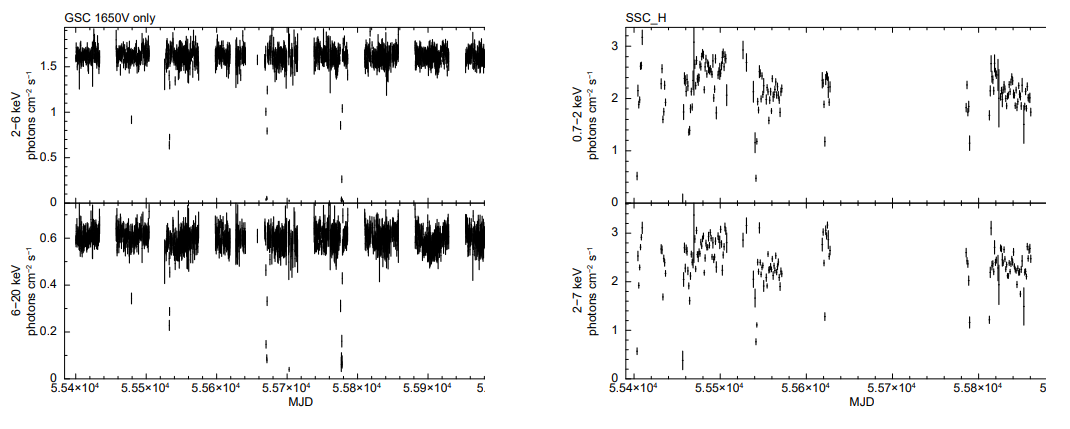
\includegraphics[width=0.95\textwidth]{4_3.png}
  \caption{Crab light curves from July 23, 2010 (MJD$=$55400) to April 23, 2012 (MJD$=$56040), a period of about a year and a half. (left): GSC 1650V counter, (right): SSC-H.}
  \label{fig:3}
\end{figure}

\section{Spectral Analysis}\label{sec:4.4}

\subsection{Extract Source and Background Energy Spectra (FITS Format)}\label{subsec:4.4.1}

Prepare a Region File for the source and background and save it in (SKY)XY coordinates referring to the explanation in \S \ref{subsec:4.3.1}. You can create and save the energy spectra of source and background using xselect as shown below. \\

\begin{lstlisting}
$ xselect
> Enter session name >[gsc4] gsc4
gsc4:SUZAKU > read events crab_gsc4_mjd55501.evt
> Enter the Event file dir >[.] .
Got new mission: MAXI
> Reset the mission ? >[yes] yes
gsc4:MAXI-GSC-32BIT > set XYNAME X Y
gsc4:MAXI-GSC-32BIT > filter region src.reg
gsc4:MAXI-GSC-32BIT > extract spec
gsc4:MAXI-GSC-32BIT > save spec crab_src.pha
Wrote spectrum to crab_src.pha
gsc4:MAXI-GSC-32BIT > clear region
gsc4:MAXI-GSC-32BIT > filter region bkg.reg
gsc4:MAXI-GSC-32BIT > extract spec
gsc4:MAXI-GSC-32BIT > save spec crab_bkg.pha
Wrote spectrum to crab_bkg.pha
\end{lstlisting}

\

When Region File is saved with (SKY)XY coordinates, the area correction parameters of selected region are reflected in BACKSCAL in the energy spectra file (FITS format). If observation time is different, or an uncommon filter is applied, it is necessary to correct Exposure and Area Factor in a different way later\footnote{Not explained in this manual.}. The method of determining background on the same detector, as described in \S \ref{subsec:4.3.1}, is not currently available for use in energy spectra analysis. It is also recommended that GSC use only 1650V data in standard analysis. The change history of GSC HV is shown in "\$CALDB/data/maxi/gsc/bcf/mx\_gsc0\_hvhist\_20100425.fits" and other documents, and is also listed in Table \ref{tab:4.2} for clarity. Look at it to find out which GSC counter is operating 1650V during the time you want to analyze.

\begin{table}[hbtp!]
\caption{The status of GSC operations (HV status) as of July 30, 2013 is shown below.}
\label{tab:4.2}
\centering
\begin{tabu} to \textwidth{lccc}
\hline \hline
\textbf{GSC}& \textbf{1650V(End Time)} & \textbf{1550V(Start Time)} & \textbf{Comment} \\
\hline
0 & 2010-04-08 18:25:00 & 2010-04-08 18:25:00 & Running at 1550V. \\
1 & 2010-11-12 15:00:00 & 2010-11-18 19:30:00 & Running at 1550V. \\
2 & 2012-04-17 17:05:00 & 2012-04-17 17:05:00 & Running at 1550V. \\
3 & 2010-04-08 18:25:00 & 2010-06-21 11:00:00 & Closed during 2010-04-08$\sim$2010-06-21. \\
4 & -- & -- & Still running at 1650V. \\
5 & -- & -- & Still running at 1650V. \\
6 & 2010-04-08 18:25:00 & -- & Closed. \\
7 & 2010-04-08 18:25:00 & 2010-04-08 18:25:00 & Running at 1550V. \\
8 & 2010-04-08 18:25:00 & 2010-04-08 18:25:00 & Running at 1550V. \\
9 & 2010-04-08 18:25:00 & -- & Closed. \\
a & 2010-04-08 18:25:00 & 2010-04-08 18:25:00 & Running at 1550V. \\
b & 2010-04-08 18:25:00 & 2010-04-08 18:25:00 & Running at 1550V. \\
\hline
\end{tabu}
\end{table}

\

\subsection{Generate Exposure Weight Map}\label{subsec:4.4.2}

\noindent\texttt{mxdetwmap}\footnote{Changed from mxobswmap, using exposure weight map in detector coordinates as an intermediate file instead of collimator coordinates.}: Calculates the Weight Map = Effective Exposure Map [cm$^2$s] of observed exposure time of the object in detector coordinate system for each camera according to observation condition file (OBSCUR file) generated in \S\ref{subsec:4.3.2}. The program is the same for both GSC and SSC. \\

\noindent\texttt{infname}: Specify the observation condition file (OBSCUR file) generated in \S\ref{subsec:4.3.2}, or a list of the files (obscur.list) as \at obscur.list.\\

\noindent\texttt{outfname}: Output file. \\

\noindent\texttt{mjd\underline{ }start}: Observation start time (MJD). Valid when a time later than the start time of input file is entered. If you enter 0, it will be the start time of the observation condition file. \\

\noindent\texttt{mjd\underline{ }end}: Observation end time (MJD). Valid when a time earlier than the end time of input file is entered. If you enter 0, it will be the end time of the observation condition file. \\

\noindent\texttt{theta\underline{ }min}: Lower limit of incidence angle $\theta_{\text{col}}$. Normally, -1.5$^{\circ}$ is specified. \\

\noindent\texttt{theta\underline{ }max}: Upper limit of incidence angle $\theta_{\text{col}}$. Normally, 1.5$^{\circ}$ is specified. \\

\noindent\texttt{phi\underline{ }min}: Lower limit of incidence angle $\phi_{\text{col}}$. Set an extra of -50$^{\circ}$. \\

\noindent\texttt{phi\underline{ }max}: Upper limit of incidence angle $\phi_{\text{col}}$. Set an extra of 50$^{\circ}$. \\

\noindent\textbf{Execution script sample for GSC/SSC} \\

\begin{lstlisting}[frame=single]

#!/bin/sh

infname="crab_gobscur_mjd55058.fits"
outfname="crab_gwmap_mjd55058.fits"
tstart=0.0
tstop=0.0
theta_min=-2.5
theta_max=2.5
phi_min=-50.0
phi_max=50.0

cmdstr="mxdetwmap $infname $outfname\
 $tstart $tstop\
 $theta_min $theta_max\
 $phi_min $phi_max"
 
echo $cmdstr
$cmdstr

\end{lstlisting}

\

\subsection{Generate RMF for Source Spectrum}\label{subsec:4.4.3}

Based on the Weight Map (Effective Exposure Map), RMF files for different incidence angles are weighted and added together to produce an RMF that is appropriate for the observation conditions of data. At the same time, EXPOSURE Keywords of source and background energy spectra (FITS format) are rewritten to Effective Exposure (cm$^2$s) by using Weight Map. The MATRIX value in RMF will now mean Efficiency\footnote{The format may change in the future.}. The program uses \texttt{mxgrmfgen} for GSC and \texttt{mxsmfgen} for SSC\footnote{Changed from mxgscrmfspec and mxsscrmfspec. Input changed to Weight Map of the detector, and GSC added parameters for HV selection and LD disable/enable.}. The input parameters are slightly different for GSC and SSC. \\

\noindent\underline{\textbf{Input parameters common to GSC and SSC}} \\

\noindent\texttt{wmapfname}: The Exposure Weight Map file generated in \S\ref{subsec:4.4.2}. \\

\noindent\texttt{specfname}: Source energy spectrum file. If there is none, specify NONE. \\

\noindent\texttt{bgdfname}: Background energy spectrum file. If there is none, specify NONE. \\

\noindent\texttt{rmfname}: Output RMF file. \\

\noindent\underline{\textbf{Input parameters for GSC only}} \\

\noindent\texttt{gsclist}: Enter the ID of GSC camera to be used in hex value [0123456789ab]. If you want to use all 12 cameras, use "0123456789ab". This is especially useful when you want to select only good quality cameras, or when you want to see data of bad cameras. Currently, GSC 3 should not be used in energy spectra analysis regardless of HV value. \\

\noindent\texttt{gscrmfdbidx}: Index file name of GSC RMF Database. \\

\noindent\texttt{dlpath}: Specify Data Downlink Path (0: LOW, 1: MED). For example, if you want to use data in \$MXDATA/gsc.v1.4/low32, specify 0 (LOW). \\

\noindent\texttt{ldcut}: LDcut. 0 (disable) or 1 (enable). \texttt{ldcut=1} forces efficiency below LD to be 0. For 1650V GSC counter data only, there is no effect at all, so specify 0. For 1550V data, LD may exceed PI=40 (2keV), so read the LD value from CALDB according to the operating mode of each counter. When analyzing mixed data of 1650V and 1550V, set ldcut=1. During spectral extraction stage, special procedures are still needed, such as cutting events below LD. Therefore, it is recommended to use only 1650V data in standard analysis. \\

\noindent\texttt{hvsel}: 1 (1650V only), 2 (1550V only), 0 (no selection). Standard analysis recommends using only data from 1650V GSC counters, so specify 1. \\

\noindent\underline{\textbf{Input parameters for SSC only}} \\

\noindent\texttt{sschz}: 0: SSC-H or 1: SSC-Z. Unlike GSC, RMFs of different cameras are not added together. \\

\noindent\texttt{quantefffile}: CALDB file for quantum efficiency. If SSC's CALDB has been installed, specify CALDB. \\

\noindent\texttt{rmfparamfile}: CALDB file for RMF Paramerter. If SSC's CALDB has been installed, specify CALDB. \\

\noindent\textbf{Execution script sample for GSC} \\

\texttt{mxgrmfgen} will synthesize an RMF File from RMF Database generated for each place on the detector's core lines and weighted by the Weight Map. To obtain RMF Database, see \S\ref{sec:3.2}. The correction of Effective Area on low energy side is performed at this stage from Crab Calibration. To support Software LD, specify low-speed system or medium-speed system. \\

\begin{lstlisting}[frame=single]

#!/bin/sh
wmapfname=crab_gwmap.fits
specfname=crab_gsc_src.pi
bgdfname=crab_gsc_bgd.pi
rmfname=crab_gscrsp.rmf
gsclist=012456789a # exclude GSC_3 and GSC_B
gscrmfdbidx=$GSCRMFDB/gscrmfdbidx.fits
dlpath=1
ldcut=1
hvsel=0

mxgrmfgen $wmapfname $specfname $bgdfname $rmfname $gsclist $gscrmfdbidx $dlpath \
$ldcut $hvsel

\end{lstlisting}

\

\noindent\textbf{Execution script sample for SSC} \\

RMF File is synthesized from CCD detector quantum efficiency and response function parameter calibration files, then weighted by the Weight Map. For SSC, separate RMF File is generated for each HZ camera. \\

\begin{lstlisting}[frame=single]

infile=crab_swmap.fits
outfile=crab_ssch.rmf
specfname=crab_ssch_src.pi
bgdfname=crab_ssch_bgd.pi
sschz=0
quantefffile=CALDB
rmfparamfile=CALDB

mxsscrmfspec $infile $outfile $specfname $bgdfname $sschz $quantefffile $rmfparamfile

\end{lstlisting}

\

\subsection{Model Fitting}\label{subsec:4.4.4}

Binning with grppha as needed, and model fitting with xspec. \\

\begin{lstlisting}
$grppha crab_gscsum_src.pi crab_gscsum_src_bin.pi
GRPPHA[] group min 100
GRPPHA[] exit
...
$ xspec
XSPEC12> read data crab_gscsum_src_bin.pi
XSPEC12> read back crab_gscsum_bgd.pi
XSPEC12> read resp crab_gscsum.rmf
XSPEC12> model wabs*pow
XSPEC12> ignore 0.0-2.0 20.0-**
XSPEC12> notice 2.0-20.0
XSPEC12> fit
...
\end{lstlisting}

\

\begin{figure}[hbtp!]
  \centering
  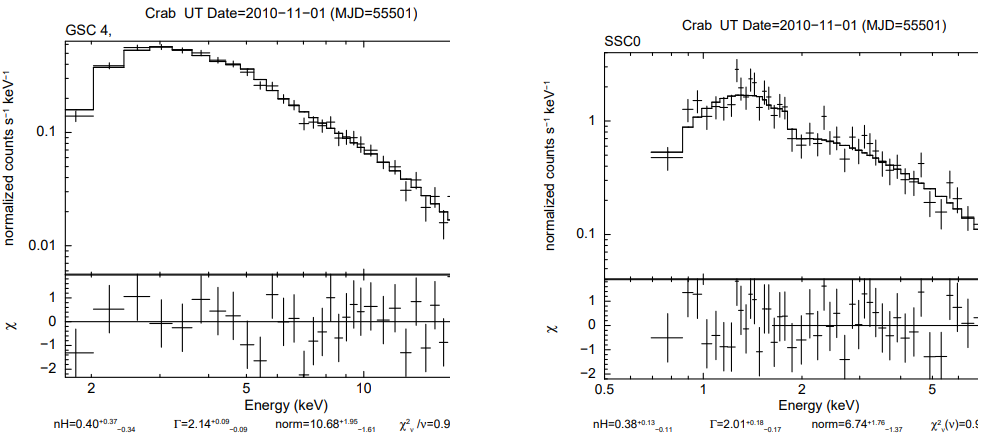
\includegraphics[width=0.95\textwidth]{4_4.png}
  \caption{Energy spectrum of Crab on November 1, 2010. (left): GSC\_4, (right): SSC\_H.}
  \label{fig:4}
\end{figure}

\section{Periodic Analysis}\label{sec:4.5}

Only GSC can perform periodic analysis. In this section, we will use Crab Pulsar as an example to explain how to analyze the period of time-varying objects such as pulsars. It basically uses xronos\footnote{http://heasarc.gsfc.nasa.gov/docs/xanadu/xronos/xronos.html} from Headas ftools package. \\

\subsection{Extracte Event Files Around the Object}\label{subsec:4.5.1}

It can be extracted in the same way as in \S\ref{subsec:4.3.1} of light curve analysis. \\

\subsection{Barycentric Correction}\label{subsec:4.5.2}

Each pulsar has its own unique pulse period. However, although pulse period from the object is constant, pulse period apparently changes due to issues on observer's side, such as MAXI's orbit around the Earth and the Earth's orbit. In order to obtain the correct pulse period from MAXI data, it is necessary to apply barycentric correction and convert it to solar system barycentric coordinate time. You can convert to solar system barycentric coordinate time with \texttt{mxbarycen}. \\

\begin{lstlisting}
$ mxbarycen
Input/output file or @filelist to be corrected[crab64.evt]
Orbit file or @orblist of the observation[@orblist.txt]
leapsec file name[Headas/heasoft-6.6.2/i686-pc-linux-gnu-libc2.5/refdata/leapsec.fits]
Right Ascension of target (NNhNNmNNs or NNN.NNN deg)[83.63]
Declination of target (+NNdNNmNNs or +NN.NNN deg)[22.01]
\end{lstlisting}

\

Currently, there is only one error that we might check. If GTI of the Event File contains zeroes, it crashes in the middle\footnote{If any other error occurs, report it to the programmer.}. In this case, you can fix it by using fv to display the Event File and delete those lines with zeroes from GTI columns. \\

\subsection{Power Spectra Analysis}\label{subsec:4.5.3}

If there is a periodic variation from the object, a peak will appear at certain frequency when FFT (Fast Fourier Transform) is performed. Use \texttt{powspec} in xronos to create a power spectrum. \\

\begin{lstlisting}
$ powspec
Ser. 1 filename +options (or @file of filenames +options)[1001_1.evt] 1001_1.evt
Name of the window file (’-’ for default window)[-] -
Newbin Time or negative rebinning[20] 0.008
Number of Newbins/Interval[8192] INDEF
Number of Intervals/Frame[15] INDEF
Rebin results? (>1 const rebin, <-1 geom. rebin, 0 none)[0] <- (*Without change*)
Name of output file[default] <- (*Without change*)
Do you want to plot your results?[yes] <- (*Without change*)
Enter PGPLOT device[/XW] <- (*Without change*)
\end{lstlisting}

\

To use default values of xronos, specify "INDEF". If there is a periodic variation, the output will be like Figure \ref{fig:5}. (30Hz)$^{-1}\simeq$0.033s, indicating that this source (Crab Pulsar) has a periodic variation of about 33ms.

\begin{figure}[hbtp!]
  \centering
  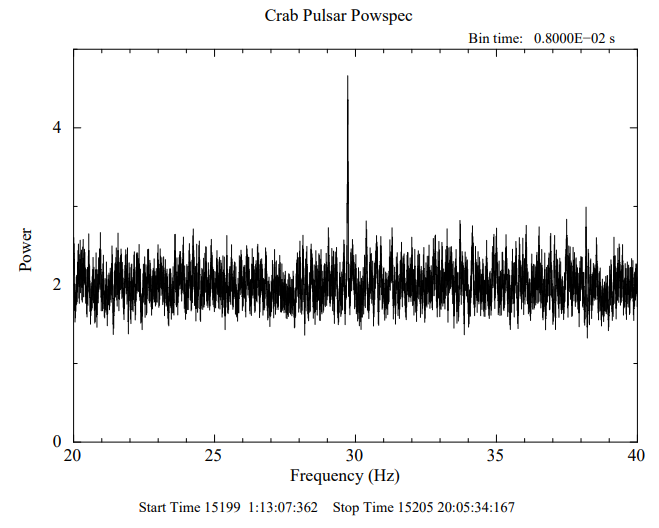
\includegraphics[width=0.65\textwidth]{4_5.png}
  \caption{The result of power spectrum output by \texttt{powspec}. The peak is seen at around 30 Hz.}
  \label{fig:5}
\end{figure}

\subsection{Periodic Search}\label{subsec:4.5.4}

Now that we know the approximate period using \texttt{powspec}, we can improve the accuracy and conduct a periodic search around that period. Use \texttt{efsearch} from xronos. For objects with monotonically increasing pulse period, such as Crab Pulsar and 4U 1626, the pulse period decay rate (ss$^{-1}$) must be specified by "efsearch dpdot=4.202E-13". Otherwise, you can skip it. \\

\begin{lstlisting}
$efsearch dpdot=4.202E-13
Ser. 1 filename +options (or @file of filenames +options)[1001_1.evt] 1001_1.evt
Name of the window file (’-’ for default window)[-] -
Epoch[0.1515500000E+05] INDEF
Period[10] 0.033
Phasebins/Period {value or neg. power of 2}[10] INDEF
Number of Newbins/Interval[38110] INDEF
Resolution for period search {value or neg. power of 2}[1E-2] 1e-10
Number of periods to search[256] 1024
Name of output file[default] <- (*Without change*)
Do you want to plot your results?[yes] <- (*Without change*)
Enter PGPLOT device[/xw] <- (*Without change*)
\end{lstlisting}

\

If it is folded with correct period, a very strong peak will appear with certain $\chi^2$ values, as shown in Figure \ref{fig:6}. However, if the pulse period is between a scan ($\sim$50s) and a revolution ($\sim$90min), fake peaks may occur at periods of (90min)$^{-1}$, 2(90min)$^{-1}$,..., so be careful when examining results. \\

\subsection{Derive Pulse Waveforms}\label{subsec:4.5.5}

Now that we know the pulse period, we can investigate waveform of the object as it fluctuates within a period. By using \texttt{efold} in xronos, a light curve with barycentric correction is convolved with pulse period. Just like \texttt{efsearch} in \S\ref{subsec:4.5.4}, specify "dpdot" option if necessary. \\

\begin{lstlisting}
$efold dpdot=4.202E-13
Number of time series for this task[1] 1
Ser. 1 filename +options (or @file of filenames +options)[kouhan.evt] 1001_1.evt
Name of the window file (’-’ for default window)[-] -
Epoch[0.1515500000E+05] INDEF
Period[249.01] 0.033
Phasebins/Period {value or neg. power of 2}[32]
Number of Newbins/Interval[121947] INDEF
Number of Intervals/Frame[1] INDEF
Name of output file[default] <- (*Without change*)
Do you want to plot your results?[yes] <- (*Without change*)
Enter PGPLOT device[/XW] <- (*Without change*)
\end{lstlisting}

\

If the pulse period is correct, pulse waveform belong to the object will output as shown in Figure \ref{fig:7}. \\

\begin{figure}[hbtp!]
  \centering
  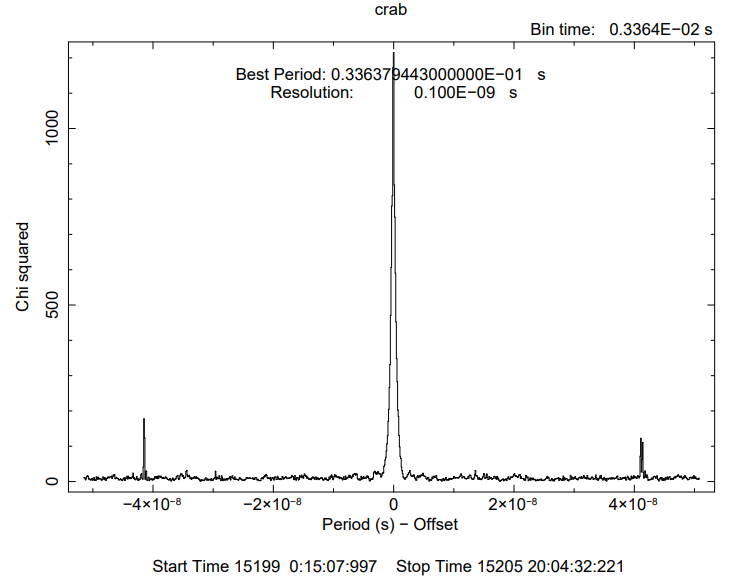
\includegraphics[width=0.6\textwidth]{4_6.png}
  \caption{The result of periodic search output by \texttt{efsearch}.}
  \label{fig:6}
\end{figure}

\begin{figure}[hbtp!]
  \centering
  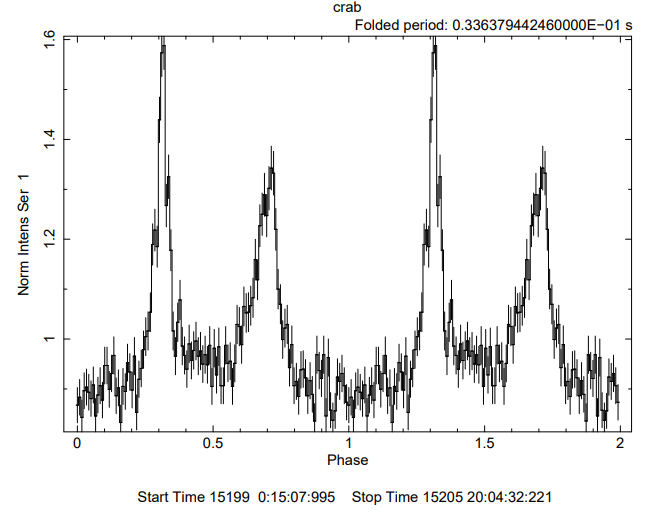
\includegraphics[width=0.6\textwidth]{4_7.png}
  \caption{Output result of convolution of barycentric corrected light curve with pulse period by \texttt{efold}.}
  \label{fig:7}
\end{figure}

\clearpage

\appendix

\chapter{Optional Software}\label{app:1}

The installation of software that is not required by standard analysis is described below. \\

\section{Install External Software}\label{appsec:1.1}

\noindent\underline{\textbf{Postgresql 8.1 or 8.2}} -- http://www.postgresql.org/ftp/source\\

\noindent \$ tar zxvf /opt/maxi/src/postgresql-8.1.23.tar.gz\\
\$ cd postgresql-8.1.23\\
\$ ./configure -{}-prefix=/opt/maxi/local 20130505\\
\$ make\\
\$ make install\\
\$ cd ../\\

\

\noindent\underline{\textbf{fftw 3.3.2}} -- ftp://ftp.fftw.org/pub/fftw/fftw-3.3.2.tar.gz\\

\noindent \$ tar zxvf fftw-3.3.2.tar.gz\\
\$ cd fftw-3.3.2 \$ ./configure -{}-prefix=/opt/maxi/local\_20130505 -{}-enable-shared\\
\$ make\\
\$ make install\\
\$ cd ../\\

\

\noindent\underline{\textbf{gsl 1.15}} -- ftp://ftp.gnu.org/gnu/gsl/gsl-1.15.tar.gz\\

\noindent \$ tar zxvf gsl-1.15.tar.gz\\
\$ cd gsl-1.15\\
\$ ./configure -{}-prefix=/opt/maxi/local\_20130505\\
\$ make\\
\$ make check\\
\$ make install\\
\$ cd ../\\

\

\noindent\underline{\textbf{HEAsoft 6.12}} -- ftp://heasarc.gsfc.nasa.gov/software/lheasoft/lheasoft6.12/heasoft-6.12src.tar.gz\\

\noindent Compile from source. For package, at least ASCA and Xspec should be selected.\\

\noindent \$ cd /opt/maxi/local\_20130505/install\_work \$ tar zxvf /opt/maxi/src/heasoft-6.12src.tar.gz\\
\$ cd heasoft-6.12/BUILD\_DIR \$ ./configure >\& config.out\\
\$ make >\& build.log\\
\$ make install >\& install.log\\

\

\noindent\underline{\textbf{ROOT 5.34.07}} -- ftp://root.cern.ch/root/root\_v5.34.07.source.tar.gz\\

\noindent If you use mxkwtool, run configure with following options.\\

\noindent \$ cd /opt/maxi/local\_20130505/install\_work \$ tar zxvf /opt/maxi/src/root\_v5.34.07.source.tar.gz \\
\$  mv root root\_v5.34.07\\
\$ cd root \_v5.34.07 \\
\$ ./configure –enable-minuit2 –enable-mathmore –enable-fftw3\\
\phantom{a}-{}-with-fftw3-incdir=/opt/maxi/local\_20130505/include\\
\phantom{a}-{}-with-fftw3-libdir=/opt/maxi/local\_20130505/lib\\
\phantom{a}-{}-with-cfitsio-incdir=\$HEADAS/include\\
\phantom{a}-{}-with-cfitsio-libdir=\$HEADAS/lib\\
\phantom{a}-{}-with-gsl-incdir=/opt/maxi/local\_20130505/include\\
\phantom{a}-{}-with-gsl-libdir=/opt/maxi/local\_20130505/lib\\
\phantom{a}-{}-with-python-incdir=/opt/maxi/local\_20130505/include/python2.7\\
\phantom{a}-{}-with-python-libdir=/opt/maxi/local\_20130505/lib\\
\$ make \\
\$ source /opt/maxi/local\_20130505/install\_work/root\_v5.34.07/bin/thisroot.csh\\
\phantom{a}/opt/maxi/local\_20130505/install\_work/root\_v5.34.07\\

\section{Install MAXI Software}\label{appsec:1.2}

\noindent\underline{\textbf{mxdbtool 2.0a}}\\

\noindent \$ cd /opt/maxi/mxsoft\_20130505 \$ mkdir mxdbtool\\
\$ cd mxdbtool\\
\$ svn export -{}-username=USERNAME http://www.maxi.jaxa.jp/svnrepo\_mission/common/mxdbtool/branches/2.0a\_c\\
\$ cd 2.0a\_c\\
\$ ./configure\\
\$ make\\
\$ make install\\

\

\noindent\underline{\textbf{mxkwtool 2.1.2}}\\

\noindent Some wcs related libraries are not included in HEAsoft 6.13, so you should specify that you want to use HEAsoft 6.12 when running configure. \\

\noindent \$ cd /opt/maxi/mxsoft\_20130505 \$ mkdir mxkwtool\\
\$ cd mxkwtool\\
\$ svn export -{}-username=USERNAME http://www.maxi.jaxa.jp/svnrepo\_mission/common/mxkwtool/branches/2.1.2\_c\\
\$ cd 2.1.2\_c\\
\$ ./configure\\
\phantom{a}-{} -with-wcs-libdir=/opt/maxi/local\_20130505/install\_work/heasoft-6.12/x86\_64-unknown-linux-gnu-libc2.12/lib\\
\$ make\\
\$ make install\\
\$ pwd\\
\phantom{a}/opt/maxi/mxsoft\_20130505/mxkwtool/2.1.2\_c\\
\$ cd ../../\\
\$ svn export -{}-username=USERNAME http://www.maxi.jaxa.jp/motoko\_maxirepos/grbtool/catalog\\

\noindent Set following environment variables to run mxkwtool.\\

\noindent \$ setenv PATH \$MXSOFT/mxkwtool/2.1.2 c/script:\$PATH\\
\$ setenv MXKWTOOL \$MXSOFT/mxkwtool/2.1.2\_c\\
\$ setenv MXKW\_TMPDIR \$HOME/maxi/tmp\\
\$ setenv MXKW\_DS9\_BIN\_DIR /opt/maxi/local\_20130505/bin\\
\$ setenv MXKW\_MXFILE\_BUSY\_FLAG \$HOME/maxi/exec\_flag\_rsync\_jax\_data\_from\_riken\\
\$ setenv MXKW\_GRBTOOL\_CAT \$MXSOFT/catalog/weblistv6\_detect091209\_merge\_t.csv\\
\$ setenv MXKW\_GRBTOOL\_CAT\_LOCAL \$HOME/maxi/srcinfo.list\\
\$ setenv LD\_LIBRARY\_PATH \$LD\_LIBRARY\_PATH:/opt/heasoft/6.12/x86\_64-unknown-linux-gnu-libc2.12/lib\\

\clearpage

\chapter{Helpful Tools}\label{app:2}
\section{Time Conversion}\label{appsec:2.1}

Using \texttt{mxtimecalc}, you can convert time between MAXI, DTPC, GPS, MJD, UTC, and JST. \\

\begin{lstlisting}
$ mxtimecalc dptc 940808110
...
DPTC Auxiliary file=/nfs/m/maxir1/maxiuser/mxdata_jax.v1/auxil/dptclist.fits
DPTC list is FITS-format.
MAXITIME = 310088096.885635
DPTC = 940808110.000000
GPS = 940808109.885635
MJD = 55132.982580
UTC Time : 2009-10-28T23:34:54.885635
JST Time : 2009-10-29T08:34:54.885635
\end{lstlisting}

\

\section{Reprocess the Processed Event File}\label{appsec:2.2}

By using mxgevt2evt, you can redo ground data processing and update Processed Event File, which equivalent to using the latest version of the software and CALDB (the feature is not fully tested yet). In the case of 32-bit, GSC-E FRC List is ignored.\\

\begin{lstlisting}
$ mxgevt2evt
Name of input event file[crab_gscall.evt]
Name of output event file[crab_gscall_new.evt]
List of attitude file[nfs/m/maxidata/jax_data/auxil_jaxa/attitude/attlist_local.txt]
List of dptc file[/nfs/m/maxidata/jax_data/auxil_jaxa/dptc/dptclist_local.txt]
Nevnets[10000] -1
phamode(0/32/64). 0: dafault (input data), 32: 32-bit evt mode, 64: 64-bit evt mode[0]
List of sys-a dptc-frc list file[/nfs/m/maxid2/jax_data/low/gscfrc/geafrcfile.fits]
List of sys-b dptc-frc list file[/nfs/m/maxid2/jax_data/low/gscfrc/gebfrcfile.fits]
...
\end{lstlisting}

\clearpage

\chapter{Positioning}\label{app:3}

The following explains the positioning method with multiple cameras and multiple scans of GSC using \texttt{mxkwtool}. Here, we use Event File obtained from Flash Report. \\

\section{Obtaine Event File}\label{appsec:3.1}

In order to perform 2D fitting, it is necessary to save Flash Report data to local PC, perform Reprocess to Rev 1.0, and convert it to ROOT File. The script to do these tasks is included in \texttt{mxkwtool}, and you can run it as follows. \\

\noindent\textbf{For CSH} \\

\begin{lstlisting}[frame=single]

set scriptdir = $MXSOFT/mxkwtool/2.1.2/script
set novaid = 6502776009
set usr = {FLASH REPORT username}
set pass = {FLASH REPORT password}
$scriptdir/get_flash_report_files.py $novaid $usr $pass |& tee getdata.log
cd $novaid

\end{lstlisting}

\

\noindent\textbf{For BASH} \\

\begin{lstlisting}[frame=single]

scriptdir=$MXSOFT/mxkwtool/2.1.2/script
novaid=6502776009
user={FLASH REPORT username}
pass={FLASH REPORT password}
$scriptdir/get_flash_report_files.py $novaid $user $pass
cd id$novaid

\end{lstlisting}

\

If the script is working correctly, a directory named id\$\{novaid\} will be created, hereafter, we will assume that you are in id\$\{novaid\}, so go to this directory. A list of Event Files for each scan under scan/fits is created in fits.list. Similarly, a list of files under att will be created in att.list, and a list of files under dptc will be created in dptc.list. \\

\section{Positioning Procedure}\label{appsec:3.2}

The following explains the procedure for positioning with multiple cameras and multiple scans. The logic is to add up the results of each camera and each scan. For positioning, set environment variables as shown in \S\ref{sec:3.6}. \\

\noindent\textbf{For CSH} \\

\begin{lstlisting}[frame=single]

set bindir = $MXSOFT/mxkwtool/2.1.2/script

set srcname = Aql_X-1
set ra = 287.816875
set dec = 0.584944
set rad = "auto"        (*\phantom{aaaaa}\# Specify the radius (deg) to create the catalog. auto means 5 deg.*)
set catfile = cat.txt   (*\# Output file name.*)
set regfile = cat.reg   (*\# Output file name.*)
set mode = sky          (*\phantom{aaaaa}\# Positioning on sky coordinates (tangent plane to the celestial sphere).*)

$bindir/mk_catalog.pl \
. \
$srcname \
$ra $dec $rad \
$catfile \
$regfile \
$mode

\end{lstlisting}

\

\noindent\textbf{For BASH} \\

\begin{lstlisting}[frame=single]

bindir=$MXSOFT/mxkwtool/2.1.2/script

srcname=Aql_X-1
ra=287.816875
dec=0.584944
rad="auto" (*\phantom{aaaaa}\# Specify the radius (deg) to create the catalog. auto means 5 deg.*)
catfile=cat.txt (*\# Output file name.*)
regfile=cat.reg (*\# Output file name.*)
mode=sky (*\phantom{aaaaaaa}\# Positioning on sky coordinates (tangent plane to the celestial sphere).*)

$bindir/mk_catalog.pl \
. \
$srcname \
$ra $dec $rad \
$catfile \
$regfile \
$mode

\end{lstlisting}

\

You should check "\$catfile"(cat.txt) generated at this stage and remove unnecessary objects. You can also remove them by changing the first character of their lines to "\#". After you remove those unwanted objects, you should re-index them (the number at the beginning of lines). However, do not delete the last line that starts with "! bg".\\
\indent The list of Event Files converted to ROOT format is written in "root.list". Since it will be used directly, make sure that the contents are written down. \\

\noindent\textbf{For CSH} \\

\begin{lstlisting}[frame=single]

set procdir = .
set root_list = root.list

set dptcfname = "auto"
set attlistfile = "auto"

set nbin_delta_sky = "auto"
set fwidth_delta_sky = "auto"

set sel_ene_lo = 4.0
set sel_ene_up = 10.0

${bindir}/detpos_sky.pl \
$procdir \
$srcname \
$root_list \
$catfile \
$dptcfname \
$attlistfile \
$nbin_delta_sky \
$fwidth_delta_sky \
$sel_ene_lo \
$sel_ene_up \
|& tee detpos_sky.log

\end{lstlisting}

\

\noindent\textbf{For BASH} \\

\begin{lstlisting}[frame=single]

procdir=.
root_list=root.list

dptcfname="auto"
attlistfile="auto"

nbin_delta_sky="auto"
fwidth_delta_sky="auto"

time ${bindir}/detpos_sky.pl \
$procdir \
$srcname \
$root_list \
$catfile \
$dptcfname \
$attlistfile \
$nbin_delta_sky \
$fwidth_delta_sky \
| tee detpos_sky.log

\end{lstlisting}

\

If you want to know the progress of aforementioned "detpos\_sky.pl" while it is running, run the following. \\

\noindent\textbf{For CSH,BASH} \\

\begin{lstlisting}[frame=single]

${bindir}/merge_cont_mklist.pl \
$procdir

${bindir}/merge_cont.pl \
$procdir \
$catfile \
$srcname

\end{lstlisting}

\

\section{Check Positioning Results}\label{appsec:3.3}

Open list.html in a web browser. You will see links to "detpos\_gpev\_id\${novaid}\_gti01\_0000\_04" and so on. You can also check Contour Plot for each scan. In "\$srcname\_cam[CAMERA-ID]\_objs.png", the initial position of the 0th object in Catalog File is displayed with a $\times$ sign. The surrounding objects are displayed like $\circ$1, $\circ$2, $\circ$3, so make sure that the number of objects matches the Catalog File. If you make a mistake when editing the Catalog File, these marks may not be displayed correctly. \\
\indent Open "merge \${srcname}/pnglist.html" in a web browser. "\${srcname}\_cont\_add.png" is the sum of two-dimensional histograms of c-stats (c-stat = --2ln(Likelihood)) of all scans. If the 2D fitting is reasonable, c-stat should be small in some areas and then increases in a circular way as it moves outward. Check if this is the case. Files such as "\${srcname}\_cont\_good\_0000.png" are two-dimensional histograms of c-stat for each scan and each camera, and should be checked for validity as well. Here is an explanation of what the numbers in files such as "\${srcname}\_cont\_good\_0000.png" represent. If multiple scans and multiple cameras are used, e.g., three scans and cam4 and cam5 data are used, "0000" is cam4 of the first scan and "0001" is cam5 of the first scan. Similarly, "0002" is followed as cam4 for the second scan.\\
\indent The fitting results of each scan should be checked and if there are any scans that are not valid, they should be removed. "cont\_hist.list" and "valid\_hist.list" list the files per scan and per camera, you can comment out those unvalidated scans with "\#". You can then run "merge\_cont.pl" to create a 2D histogram of all the scans added together, excluding those that are not valid. \\

\noindent\textbf{For CSH,BASH} \\

\begin{lstlisting}[frame=single]

emacs cont_hist.list &
emacs valid_hist.list &

${bindir}/merge_cont.pl \
$procdir \
$catfile \
$srcname

\end{lstlisting}

\clearpage

\noindent\normalfont\huge\textbf{References} \\

\

\normalsize \begin{enumerate}
  \item Heasoft Home page http://heasarc.nasa.gov/docs/software/lheasoft/
  \item CALDB Home page http://heasarc.nasa.gov/docs/heasarc/caldb/caldb\_intro.html
  \item MAXI low-speed telemetry data
  \item MAXI medium-speed telemetry data
\end{enumerate}
















\end{document}
